%%%%%%%%%%%%%%%%%%%%%%%%%%%%%%%%%%%%%%%%%%%%%%%%%%%%%%%%%%%%%
%  PREAMBLE: sets up compiler modes, loads packages, defines macros, etc
%%%%%%%%%%%%%%%%%%%%%%%%%%%%%%%%%%%%%%%%%%%%%%%%%%%%%%%%%%%%%

%%%%%%%%%%%%%%%%%%%%%%%%%%%%%%%%%%%%%%%%%%%%%%%%%%%%%%%%%%%%%
%  PREAMBLE: sets up compiler modes, loads packages, defines macros, etc
%  Steve Rodney, 2012
%%%%%%%%%%%%%%%%%%%%%%%%%%%%%%%%%%%%%%%%%%%%%%%%%%%%%%%%%%%%%


%%%%%%%%%%%%%%%%%%%%
% COMPILER MODES
%%%%%%%%%%%%%%%%%%%%

%% Set default compiler modes 
%% (these will be overridden by the -options.tex  file below, if it exists)

% Manuscript mode : 
%  True  : single-column, double-spaced, markup-ready style (with comments)
%  False : print in two-col single-space publication-ready style (no comments)
\newif\ifms
\msfalse

% Grayscale  mode : use grayscale figures when available
\newif{\ifgrayscale}
\grayscalefalse

% Changetext mode : highlight modified text in bold blue font
\newif{\ifchangetext}
\changetextfalse

%% Read in the -options.tex file (generated by the Makefile)
%%  to set the compile-mode options
\InputIfFileExists{\jobname-options}


%%%%%%%%%%%%%%%%%%%%%%%%%%%%%%%
% manuscript mode settings
%%%%%%%%%%%%%%%%%%%%%%%%%%%%%%%
\ifms
  \documentclass[manuscript]{aastex}
  \usepackage{natbib,amsmath,verbatim}
  \received{}
  \revised{}
  \accepted{}
  \citestyle{aa}
  \newcommand{\cmt}[1]{\textcolor{red}{#1}}   % Red text  for printing comments 
\else
  %\documentclass[12pt,ms,iop]{emulateapj}
  \documentclass[revtex4,iop]{emulateapj}
  \font\sevenrm=cmr7 
  \citestyle{aa} 
  \newcommand{\cmt}[1]{}
  %\slugcomment{submitted to ApJ} 
  %\journalinfo{astro-ph/xxxxxx}  % top left corner of first page.
\fi

%%%%%%%%%%%%%%%%%%%%%%%%%%%%%%%
% changetext  mode settings
%%%%%%%%%%%%%%%%%%%%%%%%%%%%%%%
\ifchangetext
  % Changed text is highlighted in bold, blue font 
  \newcommand{\change}[1]{{\bf \textcolor{blue}{#1}}}
\else
  % Changed text is indistinguishable
  \newcommand{\change}[1]{#1}
\fi


%%%%%%%%%%%%%%%%%%%%
% PACKAGES INCLUDED
%%%%%%%%%%%%%%%%%%%%
\usepackage{natbib}   % reference citations and bibliography
\usepackage{amsmath}  % extended math symbols
\usepackage{verbatim} % verbatim text formatting
\usepackage{enumerate}% enumerated lists
\usepackage{amssymb}  % extended symbols lib
%\usepackage{url}      % url text formatting
\usepackage{hyperref}      % url text formatting
\usepackage[usenames]{color}  % colored text
%\usepackage{multirow}  % muti-row table cells
%\usepackage{amsmath}  % extended equations lib (split)
%\usepackage{mathrsfs} % extended math fonts (mathscr)
%\usepackage{paralist} % inline enumeration (for Table ref lists)
%\usepackage{authblk}
\usepackage{appendix}


%%%%%%%%%%%%%%%%%%%%%%%%%%%%%%%%%%%%%%%%%%%%%%%%%%%
% PDF mode settings : Auto-select eps or pdf figures 
% based  on the compiler used (i.e. latex vs pdflatex)
%%%%%%%%%%%%%%%%%%%%%%%%%%%%%%%%%%%%%%%%%%%%%%%%%%%
\ifx\pdfoutput\undefined
  \pdffalse
  \DeclareGraphicsExtensions{.eps,.ps}
\else
  \ifnum\pdfoutput=1
    % \pdftrue
    \DeclareGraphicsExtensions{.pdf,.png,.jpg}
  \else
    % \pdffalse
    \DeclareGraphicsExtensions{.eps,.ps}
  \fi
\fi


%%%%%%%%%%%%%%%%%%%%%%%%%%%%%%%
% AUTHOR-DEFINED MACROS
%%%%%%%%%%%%%%%%%%%%%%%%%%%%%%%

% Paper aliases 
\defcitealias{Patel:2014}{P14}
\def\P14{\citetalias{Patel:2014}}

\def\tomas{HFF14Tom}

% General purpose usefulness:
\newcommand{\etal}{{et al.~}}                                             
\def\eg{{e.g.}}
\def\ie{{i.e.}}
\def\etc{{etc.}}
\newcommand{\lta}{\lesssim}                                               
\newcommand{\gta}{\gtrsim}                                                
\newcommand{\gt}{\gtsim}
\newcommand{\kms}{\,\rm km\,s^{-1}}                                       


%\def\pmstat{ \ensuremath{ \substack{ \resizebox{0.7em}{0.5em}{$\pm$} \\ \resizebox{0.7em}{0.2em}{stat}} } }
\def\pmstat{\ensuremath{\substack{\pm \\ \mbox{\scalebox{0.45}{stat}} } } }
\def\pmsyst{\ensuremath{\substack{\pm \\ \mbox{\scalebox{0.45}{syst}} } } }

% Cosmology:
\def\Om{\ensuremath{\Omega_{\rm m}}}
\def\Ot{\ensuremath{\Omega_{\rm tot}}}
\def\Ob{\ensuremath{\Omega_{\rm b}}}
\def\OL{\ensuremath{\Omega_{\Lambda}}}
\def\Ok{\ensuremath{\Omega_{\rm k}}}
\def\om{\ensuremath{\omega_{\rm m}}}
\def\ob{\ensuremath{\omega_{\rm b}}}
\def\wo{\ensuremath{w_0}}
\def\wa{\ensuremath{w_{\rm a}}}
\def\lcdm{$\Lambda$CDM}
\def\LCDM{$\Lambda$CDM}
\def\wcdm{$w$CDM}
\def\Ho{\ensuremath{H_0}}
\def\DA{\ensuremath{D_A}}
\def\DL{\ensuremath{D_L}}

% Astronomy:
\def\arcsec{\ensuremath{^{\prime\prime}}} 
\def\kms{\ensuremath{{\rm km s}^{-1}}}
\def\hgpcq{\mbox{$h^{-3}$Gpc$^3$}}
\def\hmpcq{\mbox{$h^{-3}$Mpc$^3$}}
\def\perhmpcq{\mbox{$h^{3}$Mpc$^{-3}$}}
\def\hmpc{\mbox{$h^{-1}$Mpc}}
\def\hmpci{\mbox{$h$\,Mpc$^{-1}$}}
\def\mpc{\mbox{Mpc}}
\def\mpci{\mbox{Mpc$^{-1}$}}
\def\mpcq{\mbox{Mpc$^{-3}$}}
\def\Msun{\mbox{M$_{\odot}$}}
\def\Av{\mbox{$A_V$}}
\def\Rv{\mbox{$R_V$}}

% Supernovae : 
\newcommand{\CCSN}{CC\,SN}
\newcommand{\CCSNe}{CC\,SNe}
\newcommand{\TNSN}{TN\,SN}
\newcommand{\TNSNe}{TN\,SNe}
\newcommand{\SNIa}{SN\,Ia}
\newcommand{\SNeIa}{SNe\,Ia}
\newcommand{\SNRz}{SNR($z$)}
\def\Mch{\mbox{M$_{\rm Ch}$}}
\def\Ni{\ensuremath{^{56}\mbox{Ni}}}
\newcommand{\dmfifteen}{\ensuremath{\Delta\mbox{m}_{15}}}
\newcommand{\deltamfifteen}{\ensuremath{\Delta\mbox{m}_{15}}}

% Missions:
\def\Hubble{{\it Hubble}}
\def\Hubbles{{\it Hubble's}}
\def\Spitzer{{\it Spitzer}}
\def\Chandra{{\it Chandra}}
\def\Herschel{{\it Herschel}}
\def\XMM{{\it XMM}}

% Institutions
\newcommand{\JHU}{Department of Physics and Astronomy, The Johns Hopkins University, Baltimore, MD 21218.}
\newcommand{\elsewhere}{St. Elsewhere University.}
\newcommand{\STScI}{Space Telescope Science Institute, Baltimore, MD 21218.}
\newcommand{\Berkeley}{Department of Astronomy, University of California, Berkeley, CA 94720-3411.}
\newcommand{\Riverside}{Department of Physics and Astronomy, University of California, Riverside, CA 92521.}
\newcommand{\WKU}{Department of Physics, Western Kentucky University, Bowling Green, KY 42101.}
\newcommand{\Copenhagen}{Dark Cosmology Centre, Niels Bohr Institute, University of Copenhagen, Juliane Maries Vej 30, DK-2100 Copenhagen, Denmark.}
\newcommand{\Arizona}{Department of Astronomy, University of Arizona, Tucson, AZ 85721.}
\newcommand{\SantaCruz}{Department of Astronomy and Astrophysics, University of California, Santa Cruz, CA 92064.}
\newcommand{\NotreDame}{Department of Physics, University of Notre Dame, Notre Dame, IN 46556.}
\newcommand{\TelAviv}{Department of Astrophysics, Tel Aviv University, 69978 Tel Aviv, Israel.}
\newcommand{\Rutgers}{Department of Physics and Astronomy, Rutgers, The State University of New Jersey, Piscataway, NJ 08854.}
\newcommand{\CfA}{Harvard/Smithsonian Center for Astrophysics, Cambridge, MA 02138.}
\newcommand{\Minnesota}{Department of Astronomy, University of Minnesota, 116 Church Street SE, Minneapolis, MN 55455, USA.}


%%%%%%%%%%%%%%%%%%%%%%%%%%%%%%%
% Page Setup 
%%%%%%%%%%%%%%%%%%%%%%%%%%%%%%%
\ifms
\else
  \renewcommand{\topfraction}{0.9}
  \renewcommand{\bottomfraction}{0.9}
  \renewcommand{\textfraction}{0.1}
  \renewcommand{\floatpagefraction}{0.9}
  \renewcommand{\dbltopfraction}{0.9}
  \renewcommand{\dblfloatpagefraction}{0.9}
\fi



%%%%%%%%%%%%%%%%%%%%%%%%%%%%%%%%%%%%%%%%%%%%%%%%%%%%%%%%%%%%
% MAIN DOCUMENT TEXT
%%%%%%%%%%%%%%%%%%%%%%%%%%%%%%%%%%%%%%%%%%%%%%%%%%%%%%%%%%%%

\shorttitle{A Type Ia SN Behind Abell 2744}
\shortauthors{Rodney et al.}

\begin{document}

\title{Illuminating a Dark Lens : A Type Ia Supernova \\ Magnified by Galaxy Cluster Abell 2744}

\author{Steven~A.~Rodney\altaffilmark{1,*}}
\author{Brandon Patel\altaffilmark{2}}
\author{Daniel Scolnic\altaffilmark{3}}
\author{Ryan Foley\altaffilmark{4}}
\author{Alberto Molino\altaffilmark{5,6}}
\author{Mathilde Jauzac\altaffilmark{7,8}}
\author{Gabriel Brammer\altaffilmark{9}}
\author{Marusa Bradac\altaffilmark{10}}
\author{Jose~Maria~Diego\altaffilmark{11}}
\author{Jens Hjorth\altaffilmark{12}}
\author{Or Graur\altaffilmark{13,14}}
\author{Austin Hoag\altaffilmark{10}}
\author{Saurabh Jha\altaffilmark{2}}
\author{Patrick Kelly\altaffilmark{15}}
\author{Daniel Lam\altaffilmark{16}}
\author{Julian~Merten\altaffilmark{17}}
\author{Johan Richard\altaffilmark{18}}
\author{Keren Sharon\altaffilmark{19}}
\author{Louis-Gregory Strolger\altaffilmark{9,20}}
\author{Tommaso Treu\altaffilmark{21}}
\author{Liliya Williams\altaffilmark{22}}
\author{Adi Zitrin\altaffilmark{23,*}}

\altaffiltext{1}{\JHU}
\altaffiltext{2}{\Rutgers}
\altaffiltext{3}{\Chicago}
\altaffiltext{4}{\Illinois}
\altaffiltext{5}{\CSIC}
\altaffiltext{6}{\SaoPaulo}
\altaffiltext{7}{\Durham}
\altaffiltext{8}{\KwaZulu}
\altaffiltext{9}{\STScI}
\altaffiltext{10}{\UCDavis}
\altaffiltext{11}{\IFCA}
\altaffiltext{12}{\Copenhagen}
\altaffiltext{13}{\NYU}
\altaffiltext{14}{\AMNH}
\altaffiltext{15}{\Berkeley}
\altaffiltext{16}{\HongKong}
\altaffiltext{17}{\Oxford}
\altaffiltext{18}{\CRAL}
\altaffiltext{19}{\Michigan}
\altaffiltext{20}{\WKU}
\altaffiltext{21}{\UCLA}
\altaffiltext{22}{\Minnesota}
\altaffiltext{23}{\CalTech}
\altaffiltext{*}{Hubble fellow}



\begin{abstract}
SN \tomas\ is a Type Ia Supernova (\SNIa) discovered at
$z=1.31\pm0.01$ behind the galaxy cluster Abell 2744 ($z=0.308$). This
SN has a projected separation from the cluster core of
$\sim$40\arcsec, closer to the critical lensing line than any previous
cluster-lensed \SNIa.  As such, it provides a valuable opportunity to
confront gravitational lens models of galaxy clusters with the direct
measurement of an absolute magnification at the edge of the
strong-lensing region.  We derive a tightly constrained measure of the
peak apparent magnitude, corrected for light curve shape and
exinction.  In a cosmology-independent analysis, we find that \tomas\
is \change{$0.75\pm0.15$} magnitudes brighter than unlensed \SNeIa\ at
similar redshift, implying a lensing magnification
of \change{$\mu_{\rm obs}=2.00\pm0.28$}.  We compare this direct
measurement of the magnification against predicted magnifications
from \change{14 lens models,} representing a broad range of
methodologies and incorporating a variety of strong- and weak-lensing
constraints.  The models are collectively fairly accurate: \change{
half of the models deliver median magnifications that are consistent
with the measured $\mu$ to within the 1$\sigma$ uncertainties.}
However, the models are systematically biased to higher values: none
of the tested models predict a magnification equal to or lower than
the observed $\mu$, and three models are $2-4\sigma$ above the
measured magnification.  We evaluate possible causes for this bias,
\changeG{considering both modeling errors and misinterpretation of the SN
data. Although we find no single explanation that accounts for the
entire discrepancy, we do find that the subset of ``free-form'' lens
models are more accurate and provide more realistic uncertainties than
``parametric models'' for this sight-line.} A larger sample of 10-100
lensed \SNeIa\ could provide a robust evaluation of systematic biases
in lens models.  Until such a sample exists, it is advisable
to \change{increase the estimated uncertainty of predicted
magnifications to match the dispersion observed across multiple lens
models.}
\end{abstract}

\keywords{ supernovae: general }

\section{Introduction}
\label{sec:Introduction}

\changeG{
Galaxy clusters can be used as cosmic telescopes to magnify distant
background objects through gravitational lensing, which can
substantially increase the reach of deep imaging surveys.  The lensing
magnification enables the study of objects that would otherwise be
unobservable because they are either intrinsically
faint \citep[e.g.][]{Schenker:2012,Alavi:2014} or extremely
distant \citep[e.g.][]{Franx:1997,Ellis:2001,Hu:2002,Kneib:2004,Richard:2006,Richard:2008,Bouwens:2009a,Maizy:2010,Zheng:2012,Coe:2013,Bouwens:2014,Zitrin:2014}.
Background galaxies are also {\it spatially} magnified, allowing for
studies of the internal structure of galaxies in the early universe
with resolutions of $\sim$100
pc \citep[e.g.]{Stark:2008,Jones:2010,Yuan:2011,Livermore:2015}.
}

\changeG{
Gravitational lensing can also provide a powerful window onto the {\it
transient} sky through an appropriately cadenced imaging survey.  The
flux magnification from strong-lensing clusters is especially valuable
for the study of $z>1.5$ supernovae
(SNe) \citep[e.g.]{Kovner:1988,Kolatt:1998,Sullivan:2000,Saini:2000,Gunnarsson:2003,Goobar:2009,Postman:2012},
which are still extremely difficult to characterize in unlensed
fields \citep[e.g.]{Riess:2001,Riess:2007,Suzuki:2012,Rodney:2012,Rubin:2013,Jones:2013}.
}

\changeG{
In the case of lensed SNe, we can also reverse the experimental setup:
instead of using strong-lensing clusters to study distant SNe, we can
use the SNe as tools for examining the lenses \citep{Riehm:2011}.  The
most valuable transients for testing and improving cluster lens models
would be {\it strongly lensed} SNe that are resolved into multiple
images \citep{Holz:2001,Oguri:2003}.  Transients that are lensed into
multiple images can also become cosmological tools, as the measurement
of time delays between the images can provide cosmographic information
to constrain the Hubble parameter \citep{Refsdal:1964} and other
cosmological parameters \citep{Linder:2011}.  We have recently
observed the first example of a multiply-imaged
SN \citep{Kelly:2015}, and expect to detect the reappearance of this
object (called ``SN Refsdal'') within 5 years, delivering a precise
test of lens model predictions \citep{Oguri:2015,Sharon:2015}.
Although detections of such objects are currently very
unlikely \citep{Li:2012}, they will become much more common in the
next decade \citep{Coe:2009,Dobke:2009}, and may be developed into an
important new cosmological tool.
}

\changeG{
In addition to time delays from multiply-imaged SNe, we can also
put cluster mass models to the test with the much more common category
of lensed Type Ia SNe.  
\citet[][hereafter P14]{Patel:2014} and \citet{Nordin:2014} presented
independent analyses of three lensed SNe, of which at least 2 are
securely classified as Type Ia SNe -- all found in the Cluster Lensing
and Supernova survey with Hubble (CLASH, PI:Postman, HST Program ID
12068, \citealt{Postman:2012}).  Both groups demonstrated that these
standard candles can be used to provide accurate and precise
measurements of the true absolute magnification along a random sight
line through the cluster.  Although in these cases the SNe were used
to {\it test} the cluster mass models, one could in principle
incorporate the measured magnifications of Type Ia SNe into the
cluster as additional model constraints.  In that role, Type Ia SNe
have the particular value that they can be found anywhere in the
cluster field.  Thus, they can deliver model constraints in regions of
``middle distance'' from the cluster core, where both strong- and
weak-lensing constraints are unavailable.
}

\change{
One of the key values in observing standard candles behind
gravitational lenses is \changeG{in addressing the problem of the
mass-sheet degeneracy} \citep{Falco:1985,Bradac:2004}.  This
degeneracy arises because one can introduce into a lens model an
unassociated sheet of uniform mass in front of or behind the
lens, without disturbing the primary observable quantities.  For
example, take a lens model with a given surface mass density $\kappa$,
and then transform the surface mass density to
$\kappa^{\prime}=(1-\lambda)\kappa+\lambda$ for any arbitrary value
$\lambda$.  Both the $\kappa$ and $\kappa^{\prime}$ models will
produce exactly the same values for all positional and shear
constraints from strong and weak lensing.  When lensed background
sources are available across a wide range of redshifts (as is the case
for the Abell 2744 cluster discussed here), it should in principle be
possible to account for the simplest form of a single mass sheet
within that redshift range.  However, there are more complex versions
of positional constraint
degeneracies \citep{Schneider:2014,Liesenborgs:2012}.  Such
degeneracies do not extend to the {\it absolute} magnification of a
background source's flux and size.  Therefore, an absolute measurement
of magnification from a standard candle or a standard ruler
\citep{Sonnenfeld:2011}  can break these fundamental degeneracies
\citep{Holz:2001}.
}


In Section~\ref{sec:DiscoveryAndFollowup} we present the discovery and
follow-up observations of SN \tomas\ at $z=1.31$, discovered behind the
galaxy cluster Abell 2744.  Sections~\ref{sec:Spectroscopy}
and \ref{sec:PhotometricClassification} describe the spectroscopy and
photometry of this SN, leading to a classification of the object as a
normal Type Ia SN.  In Section~\ref{sec:LightCurveFitting} we make a
direct measurement of the magnification of this source due to
gravitational lensing, and compare to predictions from lens models.
Finally, Section~\ref{sec:Discussion} discusses the tension between
our magnification measurement and the lens models, with implications
for the systematic error budget in magnification estimates for other
high-$z$ lensed sources.


\section{Discovery, Follow-up, and Data Processing}
\label{sec:DiscoveryAndFollowup}

\begin{figure*}
\begin{center}
%\includegraphics[width=\textwidth]{FIG/discovery_image}
\includegraphics[width=\textwidth]{FIG/discovery_image_lowres}
\caption{  \label{fig:DiscoveryImage} 
SN \tomas\ in the Abell 2744 field.  The left panel shows a
UV/Optical/IR color composite image constructed from all available HST
imaging of the Abell 2744 cluster field.  The inset panels on the right
show F814W imaging of the immediate vicinity of SN \tomas,
approximately 40\arcsec\ from the center of the cluster. The top panel
shows the template image, combining all data prior to the SN
appearance.  Labeled ellipses mark the nearest galaxies and their
redshift constraints: a photometric redshift for the most likely host
galaxy is marked in blue, and the spectroscopic redshift for a
background galaxy is given in yellow. The bottom panel is constructed
from all HFF F814W imaging taken while the SN was detectable, and
marks the SN location with an arrow.  (Left panel image credit: NASA,
ESA, and J. Lotz, M. Mountain, A. Koekemoer, and the HFF Team (STScI))
}
\end{center}
\end{figure*}


SN \tomas\ was discovered in Hubble Space Telescop (\HST) observations
with the Advanced Camera for Surveys (ACS) in the F606W and F814W
bands (V and i), collected on UT 2014 May 15 as part of the Hubble
Frontier Fields (HFF) survey (PI:J.Lotz,
HST-PID:13495).\footnote{\url{http://www.stsci.edu/hst/campaigns/frontier-fields}}
The HFF program is a 3-year director's discretionary initiative that
is collecting 140 orbits of HST imaging (roughly 340 ksec) on six
massive galaxy clusters, plus 6 accompanying parallel fields.
Each field is observed in 3 optical bands (ACS F435W, F606W and F814W)
and 4 infrared (IR) bands (WFC3-IR F105W, F125W, F140W, and F160W),
although the optical and IR imaging campaigns are separated by $\sim$6
months. Abell 2744 was the first cluster observed, with IR imaging
spanning 2013 October-November, and optical imaging from 2014
May-July.  A composite image of the HFF data showing the SN is
presented in Figure~\ref{fig:DiscoveryImage}.  The SN detection was
made in difference images constructed using template imaging of Abell
2744 from HST+ACS observations taken in 2009 (PI:Dupke,
HST-PID:11689).

\begin{deluxetable*}{rrlrrlrlcc}
\tablecolumns{9}
\tablecaption{\tomas\ Observations and Photometry\label{tab:Photometry}}
\tablehead{ 
    \colhead{Obs. Date}
  & \colhead{Camera}
  & \colhead{Filter}
  & \colhead{Exp. Time}
  & \colhead{Flux}
  & \colhead{Flux Err}
  & \colhead{AB Mag\tablenotemark{a}}
  & \colhead{Mag Err}
  & \colhead{AB Zero Point} 
  & \colhead{$\Delta$ZP\tablenotemark{b}} \\
    \colhead{(MJD)}
  & \colhead{}
  & \colhead{or grism}
  & \colhead{(sec)}
  & \colhead{(counts/sec)}
  & \colhead{(counts/sec)}
  & \colhead{}
  & \colhead{}
  & \colhead{} 
  & \colhead{(Vega-AB)} 
}
\startdata
56820.1 & ACS     & F435W &   5083 &   -0.149 & 0.288 &  27.66 &  \nodata  &   25.665 & -0.102\\
56821.9 & ACS     & F435W &   5083 &    0.568 & 0.287 &  28.12 &     0.55  &   25.665 & -0.102\\
56823.8 & ACS     & F435W &   5083 &    0.120 & 0.286 &  29.80 &     2.58  &   25.665 & -0.102\\
56825.0 & ACS     & F435W &   5083 &    0.115 & 0.288 &  29.85 &     2.72  &   25.665 & -0.102\\
56828.7 & ACS     & F435W &   5083 &   -0.801 & 0.289 &  27.66 &  \nodata  &   25.665 & -0.102\\
56830.9 & ACS     & F435W &   5083 &    0.544 & 0.290 &  28.16 &     0.58  &   25.665 & -0.102\\
56832.9 & ACS     & F435W &   5083 &   -0.431 & 0.288 &  27.66 &  \nodata  &   25.665 & -0.102\\
56833.9 & ACS     & F435W &   5083 &   -0.011 & 0.285 &  27.67 &  \nodata  &   25.665 & -0.102\\
56839.5 & ACS     & F435W &   5083 &   -0.118 & 0.282 &  27.68 &  \nodata  &   25.665 & -0.102\\[1mm]
56792.1 & ACS     & F606W &   5046 &    0.917 & 0.210 &  27.59 &     0.25  &   26.493 & -0.086\\
56793.0 & ACS     & F606W &   3586 &    1.750 & 0.240 &  26.89 &     0.15  &   26.493 & -0.086\\
56797.1 & ACS     & F606W &   4977 &    2.447 & 0.221 &  26.53 &     0.10  &   26.493 & -0.086\\
56800.1 & ACS     & F606W &   4977 &    2.134 & 0.215 &  26.68 &     0.11  &   26.493 & -0.086\\
56805.0 & ACS     & F606W &   5046 &    2.471 & 0.218 &  26.52 &     0.10  &   26.493 & -0.086\\[1mm]
56793.0 & ACS     & F814W &   3652 &    6.851 & 0.433 &  25.41 &     0.07  &   25.947 & -0.424\\
56797.1 & ACS     & F814W &   4904 &   14.111 & 0.589 &  24.63 &     0.05  &   25.947 & -0.424\\
56799.0 & ACS     & F814W &   5046 &   16.515 & 0.654 &  24.46 &     0.04  &   25.947 & -0.424\\
56800.1 & ACS     & F814W &   4904 &   16.111 & 0.647 &  24.48 &     0.04  &   25.947 & -0.424\\
56801.9 & ACS     & F814W &  10092 &   17.147 & 0.641 &  24.42 &     0.04  &   25.947 & -0.424\\
56803.0 & ACS     & F814W &  10092 &   18.080 & 0.670 &  24.36 &     0.04  &   25.947 & -0.424\\
56803.9 & ACS     & F814W &  15138 &   18.401 & 0.670 &  24.34 &     0.04  &   25.947 & -0.424\\
56804.1 & ACS     & F814W &   5046 &   19.470 & 0.746 &  24.28 &     0.04  &   25.947 & -0.424\\
56812.1 & ACS     & F814W &    637 &   19.666 & 1.078 &  24.27 &     0.06  &   25.947 & -0.424\\
56815.9 & ACS     & F814W &    446 &   16.831 & 1.190 &  24.45 &     0.08  &   25.947 & -0.424\\
56820.1 & ACS     & F814W &   5044 &   14.663 & 0.595 &  24.58 &     0.04  &   25.947 & -0.424\\
56821.9 & ACS     & F814W &   5044 &   14.802 & 0.600 &  24.57 &     0.04  &   25.947 & -0.424\\
56823.8 & ACS     & F814W &   5044 &   12.021 & 0.518 &  24.80 &     0.05  &   25.947 & -0.424\\
56825.0 & ACS     & F814W &   5044 &   12.792 & 0.539 &  24.73 &     0.05  &   25.947 & -0.424\\
56828.7 & ACS     & F814W &   5044 &   11.609 & 0.506 &  24.84 &     0.05  &   25.947 & -0.424\\
56830.9 & ACS     & F814W &   5044 &   10.013 & 0.462 &  25.00 &     0.05  &   25.947 & -0.424\\
56832.9 & ACS     & F814W &   5044 &    9.743 & 0.453 &  25.03 &     0.05  &   25.947 & -0.424\\
56833.9 & ACS     & F814W &   5044 &    9.987 & 0.462 &  25.00 &     0.05  &   25.947 & -0.424\\
56839.5 & ACS     & F814W &   5044 &    6.993 & 0.390 &  25.39 &     0.06  &   25.947 & -0.424\\[1mm]
56833.1 & WFC3-IR & F105W &    756 &   23.317 & 0.742 &  24.10 &     0.09  &   26.269 & -0.645\\
56841.8 & WFC3-IR & F105W &    756 &   18.090 & 0.648 &  24.40 &     0.11  &   26.269 & -0.645\\
56850.1 & WFC3-IR & F105W &    756 &   12.281 & 0.643 &  24.77 &     0.12  &   26.269 & -0.645\\
56860.6 & WFC3-IR & F105W &   1159 &    9.008 & 0.520 &  25.13 &     0.12  &   26.269 & -0.645\\
56886.6 & WFC3-IR & F105W &   1159 &    3.779 & 0.458 &  26.09 &     0.22  &   26.269 & -0.645\\
56891.7 & WFC3-IR & F105W &    356 &    3.018 & 1.007 &  26.34 &     0.34  &   26.269 & -0.645\\
56893.2 & WFC3-IR & F105W &    712 &    2.965 & 0.753 &  26.33 &     0.32  &   26.269 & -0.645\\
56954.6 & WFC3-IR & F105W &    356 &    1.618 & 1.206 &  27.01 &     0.65  &   26.269 & -0.645\\[1mm]
56817.1 & WFC3-IR & F125W &   1206 &   27.248 & 0.615 &  23.92 &     0.06  &   26.230 & -0.901\\
56833.2 & WFC3-IR & F125W &    756 &   24.972 & 0.822 &  24.01 &     0.06  &   26.230 & -0.901\\
56841.8 & WFC3-IR & F125W &    806 &   19.374 & 0.733 &  24.29 &     0.07  &   26.230 & -0.901\\
56850.1 & WFC3-IR & F125W &    806 &   13.989 & 0.722 &  24.64 &     0.09  &   26.230 & -0.901\\[1mm]
56891.9 & WFC3-IR & F140W &    712 &    6.770 & 0.903 &  25.42 &     0.19  &   26.452 & -1.076\\
56893.1 & WFC3-IR & F140W &    712 &    9.551 & 0.868 &  25.06 &     0.14  &   26.452 & -1.076\\
56955.6 & WFC3-IR & F140W &   1424 &    3.199 & 0.707 &  26.25 &     0.23  &   26.452 & -1.076\\[1mm]
56817.1 & WFC3-IR & F160W &   1206 &   20.211 & 1.102 &  24.27 &     0.09  &   25.946 & -1.251\\
56833.2 & WFC3-IR & F160W &    756 &   16.591 & 1.007 &  24.46 &     0.10  &   25.946 & -1.251\\
56841.8 & WFC3-IR & F160W &    756 &   12.599 & 0.978 &  24.76 &     0.10  &   25.946 & -1.251\\
56850.1 & WFC3-IR & F160W &    756 &   11.482 & 0.933 &  24.86 &     0.13  &   25.946 & -1.251\\
56860.7 & WFC3-IR & F160W &   1159 &    7.927 & 0.740 &  25.26 &     0.16  &   25.946 & -1.251\\
56886.6 & WFC3-IR & F160W &   1159 &    7.018 & 0.800 &  25.40 &     0.16  &   25.946 & -1.251\\[1mm]
\tableline\\
56812.0 & ACS     & G800L &   3490 &  \nodata & \nodata & \nodata & \nodata & \nodata & \nodata\\
56815.7 & ACS     & G800L &   6086 &  \nodata & \nodata & \nodata & \nodata & \nodata & \nodata
\enddata
\tablenotetext{a}{For non-positive flux values we report the magnitude as a 3-$\sigma$ upper limit}
\tablenotetext{b}{Zero point difference: the magnitude shift for conversion from AB to Vega magnitude units.}
\end{deluxetable*}






\begin{figure}
\begin{center}
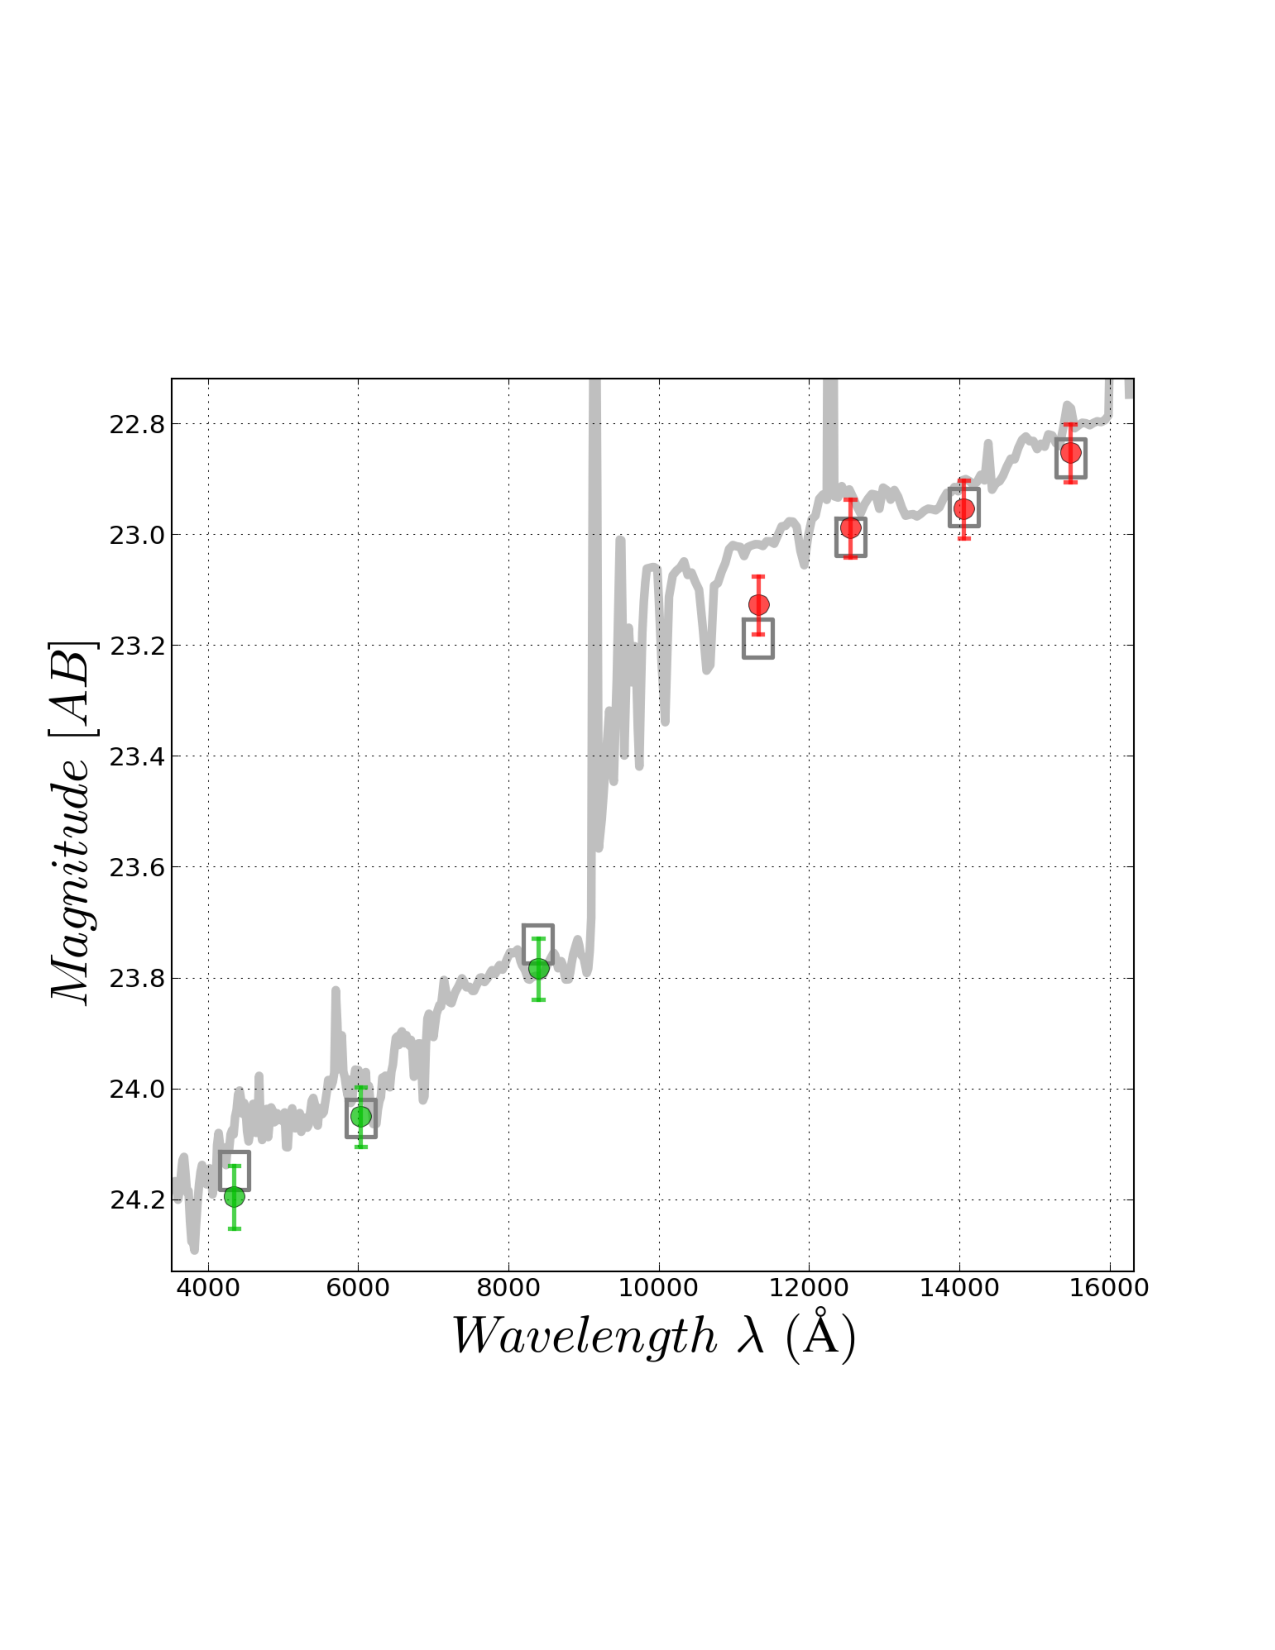
\includegraphics[width=\columnwidth]{FIG/host_sed_fit}
\caption{  \label{fig:HostSED}
Best-fit SED template match for the most probable \tomas\ host
galaxy. Using the {\it BPZ} code to match the observed SED, we find
the nearest galaxy to the SN position is a late type galaxy with a
photometric redshift of $z=1.5\pm0.2$.}
\end{center}
\end{figure}

The most probable host galaxy for SN \tomas\ is a faint and diffuse
galaxy immediately to the south-east of the SN location.  With
photometry of the host galaxy collected from the template images, we
fit the spectral energy distribution (SED) using the {\it BPZ} code --
a Bayesian photometric redshift estimator \citep{Benitez:2000}. The
best-fit SED template match is shown in Figure~\ref{fig:HostSED}.
From the {\it BPZ} analysis, we found the host to be most likely an
actively star-forming galaxy at a redshift of $z=1.5\pm0.2$.  

Another nearby bright galaxy to the East of the SN has a spectroscopic
redshift of $z=1.742$.  This redshift was determined from a spectrum
taken with the G141 grism of the HST WFC3-IR camera, collected as part
of the Grism Lens Amplified Survey from Space (GLASS, PI:Treu,
PID:13459, \citealt{Treu:2015}). \change{As we will see in Sections~\ref{sec:Spectroscopy}
and \ref{sec:PhotometricClassification}, the SN data are inconsistent
with that redshift, meaning that this nearby galaxy is a background
object and therefore has no impact on the SN magnification.}

Upon discovery, HST target-of-opportunity observations were triggered
from the FrontierSN program (PI:Rodney, HST-PID:13386), which aims to
discover and follow transient sources in the HFF cluster and parallel
fields. The FrontierSN observations provided WFC3-IR imaging as well
as spectroscopy using the ACS G800L grism, supplementing the
rapid-cadence optical imaging from HST+ACS already being provided by
the HFF program. \change{The last detections in the IR F105W and F140W
bands came from the direct-imaging component of the GLASS program}.
Difference images for the IR follow-up data were generated using
templates constructed from the HFF WFC3-IR imaging campaign, which
concluded in November, 2013.

All of the imaging data were processed using the {\tt sndrizpipe}
pipeline,\footnote{\url{https://github.com/srodney/sndrizpipe} v1.2
DOI:10.5281/zenodo.10731} a custom data reduction package in Python
that is employs the {\tt DrizzlePac} tools from the Space Telescope
Science Institute (STScI) \citep{Fruchter:2010}.  Photometry was
collected using the {\tt PyPhot} software
package,\footnote{\url{https://github.com/djones1040/PyPhot}} a
pure-Python implementation of the photometry algorithms from the IDL
AstroLib package \citep{Landsman:1993}, which in turn are based on the
DAOPHOT program \citep{Stetson:1987}.  For the IR bands we used point
spread function (PSF) fitting on the difference images, and in the ACS
optical bands we collected photometry with a
0\farcs3 aperture. Table~\ref{tab:Photometry} presents the list of
observations, along with measured photometry from all available
imaging data.
 


\section{Spectroscopy}
\label{sec:Spectroscopy}

\begin{figure}
\begin{center}
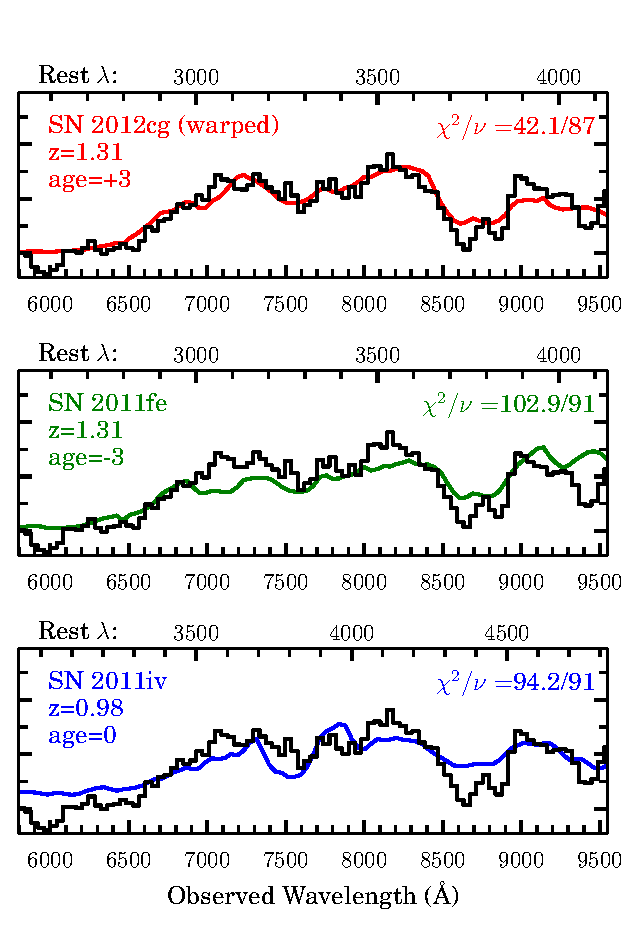
\includegraphics[width=\columnwidth]{FIG/specfit}
\caption{  \label{fig:SpecFit}
Redshift and age determination from spectral template matching to the
the SN \tomas\ maximum light spectrum.  The y axis plots flux in
arbitrary units, and the x axis marks wavelength in \AA\ with the
observer-frame on the bottom and rest-frame on the top.
The \tomas\ spectrum observed with the
HST ACS G800L grism is shown in black, overlaid with model fits
derived from a library of Type Ia templates that have extended
rest-frame UV coverage.  {\it Top}: The best match is at $z=1.31$ with
age=$+3$ days, from the normal Type Ia SN 2012cg template when using a
smooth 3rd-order polynomial to warp the shape of the template
pseudo-continuum.  When the templates are not warped, an acceptable
fit can be found with a normal Type Ia at $z=1.31$ (middle) or at
$z\sim1$ (bottom), although the latter is inconsistent with the host
galaxy redshift prior and the light curve. No \CCSN\ templates can
provide a statistically acceptable fit at any redshift, within the age
constraints imposed by the light curve.}
\end{center}
\end{figure}


A spectrum of SN \tomas\ was collected with the ACS G800L grism on
2014 June 4 and 7, when the SN was very near to its peak brightness.
The observations -- listed at the bottom of Table~\ref{tab:Photometry}
-- used 5 HST orbits from the FrontierSN program for a total
spectroscopic exposure time of $\sim$10 ksec.  The grism data were
processed and the target spectrum was extracted using a custom
pipeline \citep{Brammer:2012}, which was developed for the 3D-HST
program (PI:Van Dokkum; PID:12177, 12328) and also used by the Grism
Lens Amplified Survey from Space (GLASS; PI:Treu; PID:13459).

Figure~\ref{fig:SpecFit} shows the composite 1-D ACS grism spectrum,
combining all available G800L exposures, overlaid with SN model fits
that will be described below.  The spectrum is largely free of
contamination, because the orientation was chosen to avoid nearby
bright sources and the host galaxy is diffuse and optically faint.
Thus, the SN spectral features can be unambiguously identified, most
notably the red slope of the continuum and a prominent absorption
feature at $\sim$8700\AA.  However, the signal to noise ratio (S/N)
for the host galaxy spectrum was too weak to yield any additional
constraints on the host type or redshift.

\changeG{
Spectra of Type I SNe (including all sub-classes Ia, Ib and Ic) are
dominated by broad absorption features, which cannot in general be
used to directly extract a spectroscopic redshift \citep[see
e.g.][]{Filippenko:1997}.  As described below, we fit template spectra
to the SN \tomas\ data in two steps.}  First we determine a spectral
classification -- and get a preliminary estimate of the redshift and
age -- using the SuperNova IDentification (SNID)
software \citep{Blondin:2007}.  Second, we refine the redshift and age
measurement using a custom Type Ia spectral template matching program.

\subsection{Classification with SNID}
\label{sec:SNID}

The SNID program is designed to estimate the type, redshift, and age
of a SN spectrum through cross-correlation matching with a library of
template spectra, \change{using the algorithm of \citet{Tonry:1979}.}
To account for possible distortions in the broad shape of the SN
pseudo-continuum due to dust or instrumental calibration effects, SNID
divides each SED by a smooth cubic spline fit. This effectively
removes the shape of the SN pseudo-continuum to leave behind a flat
SED superimposed with spectral absorption and emission features.  It
is these features which drive the cross-correlation fit, so the SNID
approach is insensitive to the overall color of the SED.  We used v2.0
of the SNID template library, which includes template SEDs covering
all Type Ia and Core Collapse sub-classes, and has recently been
updated with corrections and improvements to the Type Ib/c
templates \citep{Liu:2014}.

In SNID the goodness of fit is evaluated primarily through the {\it
rlap} parameter, which measures the degree of wavelength overlap and
the strength of the cross-correlation peak.  Typically, an {\it rlap}
value $>5$ is required to be considered an acceptable match.  

To match the SN \tomas\ spectrum we use conservative constraints on
age and redshift: limiting the age to $\pm$5 rest-frame days of peak
brightness and $0.8<z<1.8$, consistent with the SN light curve and
host galaxy photo-$z$.  With these constraints we find that the only
acceptable match is a normal Type Ia SN near $z=1.3$. The best match
has {\it rlap}$=8.7$, using the normal Type Ia SN 2005cf at $z=1.35$
and age=-2.2 rest-frame days before peak.  Within these constraints,
the best non-Ia matches all have {\it rlap}$<2.5$.

Using {\tt SNID} we can find an acceptable \CCSN\ match only
when we remove all age and redshift constraints. In this case the best
non-Ia match is the Type Ic SN 1997ef, which delivers {\it rlap}$=6.8$
at $z=0.51$ and age=47.3 rest-frame days past peak.  This is not as
good a fit as the best Type Ia models, is at odds with the host galaxy
redshift prior, and is strongly disfavored by the shape and colors of
the SN light curve (see Section~\ref{sec:PhotometricClassification}).  

From the preceding analysis, we conclude that \tomas\ is a Type Ia SN
at $z\approx1.3$.  At this redshift, the absorption at $\sim$8700\AA\
corresponds to the blended \ion{Ca}{2} H\&K features.
This \ion{Ca}{2} absorption is commonly seen in Type Ia SN spectra
near maximum light, although it is also prominent in the spectra of
Type Ib and Ic core collapse SNe (\CCSNe).  The red color of
the \tomas\ SED is qualitatively consistent with a redshift of $z>1$
-- although this information was not used by {\tt SNID} for the
template matching.  As we will see in Section~\ref{sec:PhotometricClassification},
this spectral classification of SN \tomas\ is reinforced by the
photometric information, which also supports classification as a Type
Ia SN at $z\approx1.3$.


\subsection{Spectroscopic Redshift}
\label{sec:SpecRedshift}

To refine the redshift and phase constraints on \tomas, we next fit
the spectrum with a custom spectral matching program that employs a
library of Type Ia SN SEDs.  This library is similar to the Type Ia
spectral set used by SNID, but also includes more recent SNe with
well-observed spectral time series that extend to rest-frame UV
wavelengths (e.g. SN 2011fe and 2014J).  We first use an approach
similar to the SNID algorithm: warping the pseudo-continuum of each
template spectrum by dividing out a 3$^{\rm rd}$-order polynomial to
match the observed SED of SN \tomas.  From this analysis we find
results that are consistent with the SNID fits: a redshift of
$z=1.31\pm0.01$ and a phase of $0\pm3$ rest-frame days. The
best-fitting spectral template is the normal Type Ia SN 2012cg, shown
in the top panel of Figure~\ref{fig:SpecFit}, which has $\chi^2$
per degree of freedom $\nu$ equal to 42.1/87.

Finally, we repeat the fitting, but without any warping of the
templates to account for differences in the continuum shape.  In this
iteration we only allow each template SED to be scaled in flux
coherently at all wavelengths.  As shown in Figure~\ref{fig:SpecFit},
we again find that the \tomas\ SED can be matched by a normal Type Ia
SN (SN 2011fe) at redshift $z=1.31\pm0.01$.  Without the continuum
warping, an alternative fit also arises: the \change{fast-declining
(91bg-like)} Type Ia SN 2011iv
at $z=0.98\pm0.01$. Formally, this match provides a slightly better
fit to the unwarped \tomas\ spectrum, although the fit is notably poor
at $\sim8700$\AA\ where the most significant absorption feature is
found. Furthermore, a redshift $z\sim1$ is at odds with the host
galaxy photo-z ($1.5\pm0.2$), and we will see in the following section
that the photometric data is also incompatible with a Type Ia SN at
$z\sim1.0$.

Setting aside the $z\sim1$ solution, all other template matches
provide a consistent redshift constraint of $z=1.31\pm0.01$,
regardless of whether the templates are warped to match the SN \tomas\
continuum shape.  The inferred age from these fits is $0\pm3$
rest-frame days from peak brightness, which is also consistent with
the observed light curve.


\section{Photometric Classification}
\label{sec:PhotometricClassification}

Relative to other SNe at $z>1$, the SN \tomas\ light curve was
unusually well sampled at rest-frame ultraviolet wavelengths, due to
the rapid cadence of the HFF imaging campaign. These ACS observations
therefore provide a tight constraint on the time of peak brightness
and the evolution of the SN color.  Supplemental observations with the
WFC3-IR camera provided critical rest-frame optical photometry,
enabling a measurement of the apparent luminosity distance through
light curve fitting.

\begin{figure}
\begin{center}
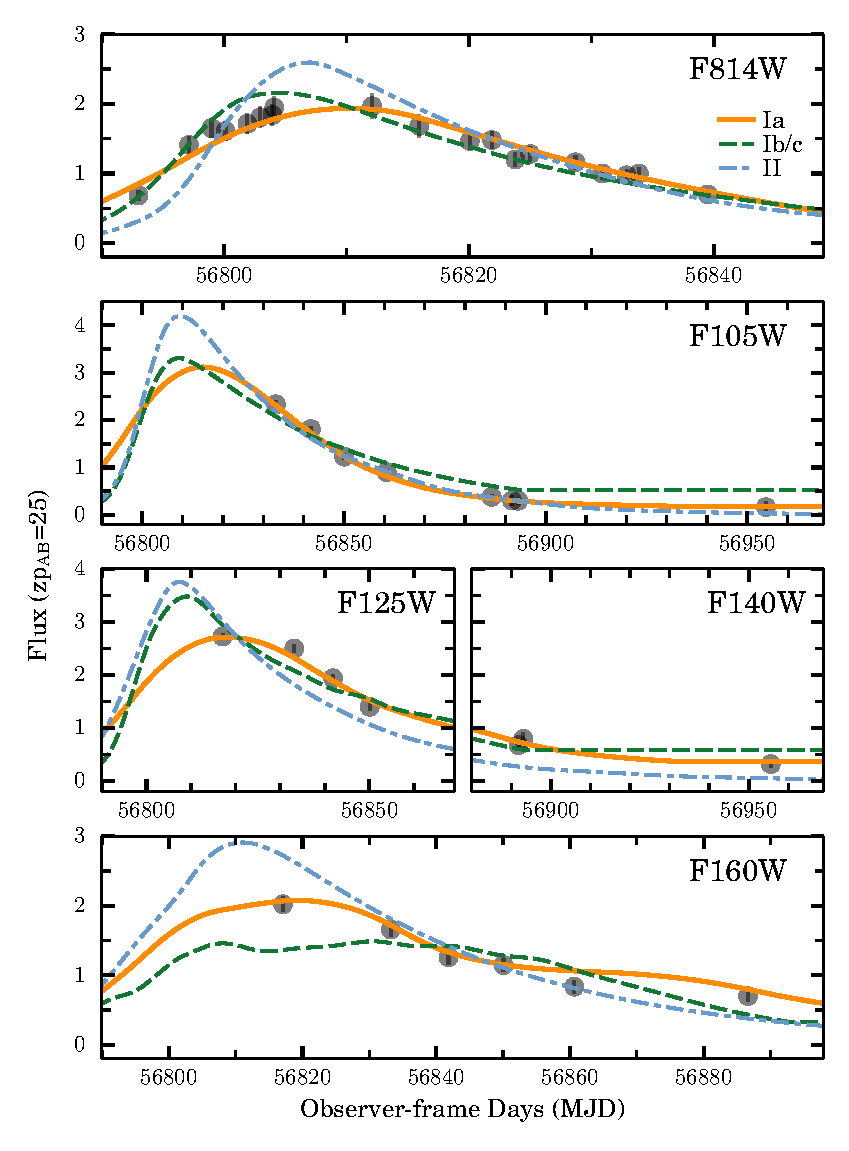
\includegraphics[width=\columnwidth]{FIG/snTomas_lightcurve_classification}
\caption{ 
Maximum likelihood model for each SN sub-class, derived from Bayesian
model selection using the photometric data alone. Grey points show the
observed SN \tomas\ photometry with error bars, though these are typically
smaller than the size of the marker.  The Type Ia model
(orange solid line) is drawn from the SALT2 template at $z=1.35$. The
best match from all Type Ib/Ic models is based on the Type Ic SN
SDSS-14475 at $z=0.695$ (green dashed line). For the Type II class, the
best match is from the Type II-L SN 2007pg at $z=1.8$ (blue dash-dot line). The Type
Ia model is by far the best match, and the only one that is consistent
with both the photo-$z$ of the probable host galaxy and the
spectroscopic redshift from the SN spectrum.
\label{fig:photoclass} }
\end{center}
\end{figure}

As a check on the spectral classification of SN \tomas\
(Section~\ref{sec:SNID}), we independently classified the SN using a
Bayesian photometric classifier.  We use the
{\tt sncosmo} software
package\footnote{\url{http://sncosmo.github.io/}} to simulate SN light
curves from $z=0.3$ to 2.3 and evaluate the classification
probability using traditional Bayesian model selection \citep[as
in][]{Jones:2013,Rodney:2014,Graur:2014,Rodney:2015a}.  In this
analysis we represent normal Type Ia SNe with the SALT2
model \citep{Guy:2010}, and \CCSNe\ with 42 discrete templates (26
Type II and 16 Type Ib/c) drawn from the template library of the
SuperNova Analysis software
package \citep[SNANA,][]{Kessler:2009a}.\footnote{Throughout this work
we use SNANA v10\_35g.}
Likelihoods are defined by comparing the observed fluxes to model
predictions in all passbands where the model is defined.  In practice,
this means we exclude the F435W and F606W bands, which are too blue
for our models at $z>0.85$.

The \CCSN\ models have free parameters for date of peak brightness
($t_{\rm pk}$), amplitude, and redshift ($z$). Due to the expected
impact of gravitational lensing magnification, we do not include any
prior on the intrinsic luminosity for any SN sub-class.  We also do
not assign a prior for the SN redshift. This allows our photometric
analysis to provide an independent check on the host galaxy photo-$z$
and spectroscopic redshift (Sections~\ref{sec:DiscoveryAndFollowup}
and \ref{sec:SpecRedshift}).

For Type Ia SNe, the SALT2 model has two additional parameters that
control the shape ($x_1$) and color ($c$) of the light curve.  We use
conservative priors here, defined to encompass a range of Type Ia SN
shapes and colors that is broader than typically allowed in
cosmological analyses \citep[see
e.g.,][]{Kessler:2009b,Sullivan:2011,Rest:2014}. For $x_1$ the prior is
a bifurcated Gaussian distribution with mean $\bar{x}_1=0$, dispersion
$\sigma_{x_1}^+={0.9}$ and $\sigma_{x_1}^-={-1.5}$.  The prior for the
color parameter $c$ has $\bar{c}=0.0$, $\sigma_c^-=0.08$, and
$\sigma_c^+=0.54$.  The $c$ parameter in SALT2 combines intrinsic SN
color and extinction due to dust, so the large red tail of this
distribution allows for the possibility of several magnitudes
of dust extinction along the \tomas\ line of sight.

We also assign a class prior for each of the three primary SN
sub-classes (Type Ia, Ib/c, and II), using a fixed relative fraction for
each sub-class as determined at $z=0$ by \citet{Smartt:2009}
and \citet{Li:2011a}.  A more rigorous classification would extrapolate
these local SN class fractions to higher redshift using models or
measurements of the volumetric SN rate.  For simplicity, we do not
vary the class priors with redshift, and in practice these priors do
not have any significant impact on the resulting classification.

The final photometric classification probability for SN \tomas\ is
$p({\rm Ia}|{\rm {\bf D}})=1.0$, with the classification probability
from all \CCSN\ sub-classes totaling less than
$10^{-32}$.  \change{Although this Bayesian classification utilizes
the full posterior probability distribution, for illustration we
highlight in Figure~\ref{fig:photoclass} a single best-fit model for
each sub-class.} This demonstrates how the \CCSN\ models fail to
adequately match the observed photometry. In particular, only the Type
Ia model can simultaneously provide an acceptable fit to the
well-sampled rising light curve in F814W and the F814W-F160W color
near peak.

The marginal posterior distribution in redshift for the Type Ia model
is sharply peaked at $z=1.35\pm0.02$, which is fully consistent with
the photo-$z$ of the presumed host galaxy ($z=1.5\pm0.2$), and
$<2\sigma$ from the spectroscopic redshift of $z=1.31\pm0.01$ derived
in Section~\ref{sec:SpecRedshift}.  The time of peak brightness is
also tightly constrained at $t_{\rm pk}=56816.3\pm0.3$, which means
the spectroscopic observations were collected within 2 rest-frame days
of the epoch of peak brightness, consistent with our spectroscopic
analysis.


\section{Light Curve Fitting}
\label{sec:LightCurveFitting}

With the spectroscopic type and redshift securely defined as a normal
Type Ia SN at $z=1.31$, we now turn to fitting the light curve with
Type Ia templates to measure the distance modulus.  Here we use two
independent light curve fitters: the SALT2 model described
above and the MLCS2k2 model \citep{Jha:2007}.   


\begin{figure*}
\begin{center}
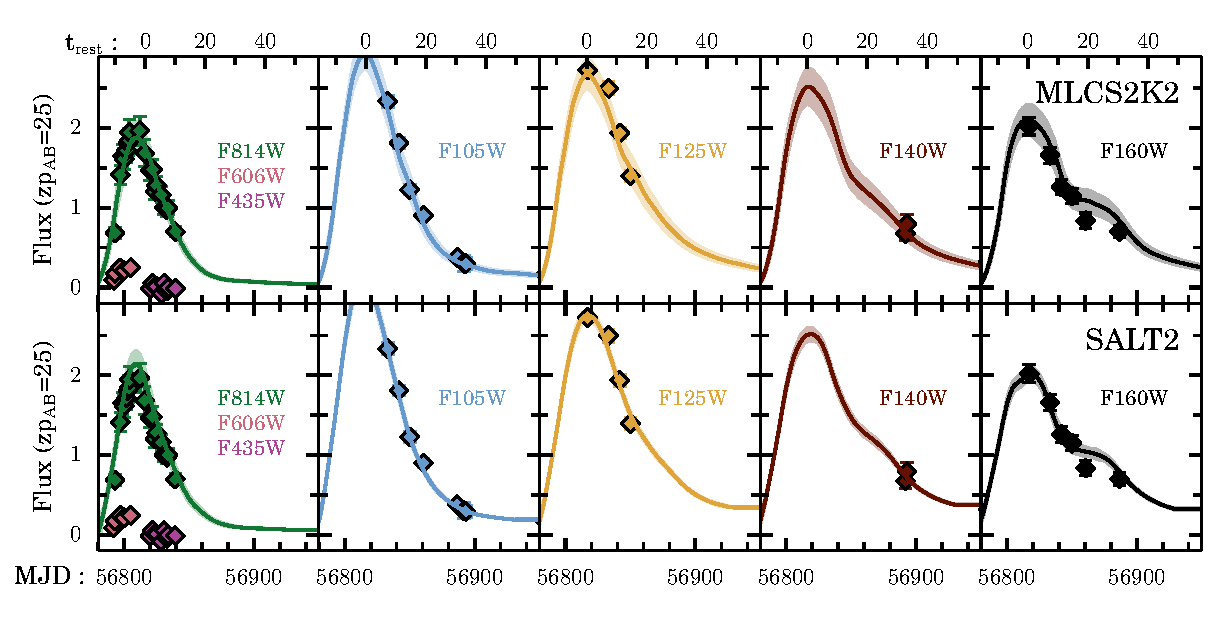
\includegraphics[width=\textwidth]{FIG/snTomas_lightcurve_fit_fluxAB25}
\caption{ Type Ia light curve fits to SN \tomas\ using the MLCS2k2
(top row) and SALT2 (bottom row) fitters. The model redshifts are set to
$z=1.33\pm0.02$, encompassing both redshift values as determined from
spectroscopic and photometric constraints.  Solid lines denote the
best-fit model and shaded lines show the range allowed by 1-$\sigma$
uncertainties on the model parameters. 
Observed fluxes are shown as diamonds, scaled to an AB magnitude
zero point of 25. Error bars are plotted, but most are commensurate
with the size of the points. The left-most panel includes observations
in the F435W and F606W filters, although these were not used for the
fit, as they are bluer than the minimum wavelength for the model. The
lower axis marks time in observer frame days, while the top axis shows
the time in the rest frame relative to the epoch of peak brightness.
\label{fig:LightCurveFits} }
\end{center}
\end{figure*}

With both fitters we find light curve shape and color parameters that
are fully consistent with a normal Type Ia SN, regardless of whether
we adopt the spectroscopic redshift $z=1.31$ from
Section~\ref{sec:SpecRedshift} or the photometric redshift $z=1.35$
from Section~\ref{sec:PhotometricClassification}.  For SALT2, with the
redshift range set to $1.33\pm0.02$, we find a light curve shape
parameter of $x_1=0.164\pm0.199$ and a color parameter of
$c=-0.115\pm0.025$, yielding a $\chi^2$ value of 48.4 for 36 degrees
of freedom, $\nu$.  With the MLCS2k2 fitter the best-fit shape
parameter is $\Delta=-0.033\pm0.083$ and the color term is
$A_{\rm V}=0.014\pm0.037$, giving $\chi^2/\nu=23.9/36$.

\subsection{Distance Modulus}
\label{sec:DistanceModulus}

As in \P14, we derive a distance modulus\footnote{We use 'dm' to
indicate the distance modulus to avoid confusion, reserving the symbol
$\mu$ to refer to the lensing magnification. This 'dm' is a standard
distance modulus, defined as ${\rm dm}=5\log_{10}d_L+25$, where $d_L$
is the luminosity distance in Mpc.} \changeG{while ignoring the
effects of gravitational lensing, so that we can later use it to
derive a direct measurment of the magnification.}  From the SALT2 fit
we get

\begin{equation} \label{eqn:dmSALT2}
 {\rm dm}_{\rm SALT2} = m_B^* - M + \alpha(s-1) - \beta C.
\end{equation}

\noindent  Here the parameters for light curve shape $s$ and color $C$ 
correspond to the SiFTO light curve fitter \citep{Conley:2008}, so we
first use the formulae from \citet{Guy:2010} to convert from SALT2
($x_1$ and $c$) into the equivalent SiFTO parameters.  We also add an
offset of 0.27 mag to the value of $m_B^*$ returned by SNANA, in order
to match the arbitrary normalization of the SALT2 fitter used
by \citet{Guy:2010} and \citet{Sullivan:2011}.  This conversion allows
us to adopt values for the constants $M$, $\alpha$, and $\beta$
from \citet{Sullivan:2011}, which have been calibrated using 472 SNe
from the SNLS3 sample \citep{Conley:2011}: $M=-19.12\pm0.03$,
$\alpha=1.367\pm0.086$, and $\beta=3.179\pm0.101$.

\begin{deluxetable}{lccc}
\tablecolumns{4}
\tablecaption{\tomas\ Measured Magnification\label{tab:MeasuredMagnification}}
\tablehead{ 
    \colhead{}
  & \multicolumn{2}{c}{Distance Modulus}
  & \colhead{Measured}\\
    \colhead{Fitter}
  & \colhead{\tomas}
  & \colhead{Control}
  & \colhead{Magnification}
}
\startdata
MLCS2k2  & $44.06\pm0.09$ & $44.81\pm0.05$ & $2.00\pm0.19$\\
SALT2    & $44.09\pm0.16$ & $44.78\pm0.05$ & $1.89\pm0.29$
\enddata
\end{deluxetable}






The SNANA version of the MLCS2k2 fitter returns a value for the
distance modulus (dm$_{\rm MLCS2k2}$) that has an arbitrary zero point
offset relative to the SALT2 distances (dm$_{\rm SALT2}$).  To put the
two distances onto the same reference frame we add a zeropoint
correction of 0.20 mag to the MLCS2k2 distances as
in \P14.  This correction was derived by applying both
fitters to a sample of Type Ia SNe from the SDSS
survey \citep{Holtzman:2008,Kessler:2009b}, with the extinction law
$R_V$ fixed at 1.9.

\change{
The total uncertainty in the distance modulus is  
}

\begin{equation} \label{eqn:sigmatot}
 \sigma_{\rm tot} = \sqrt{ \sigma_{\rm stat}^2 + \sigma_{int}^2}.
\end{equation}

\change{
\noindent
The $\sigma_{\rm stat}$ term is the statistical uncertainty, which
encapsulates uncertainties from the data and the model, and
$\sigma_{\rm int}$ accounts for the remaining {\it unmodeled} scatter.
This latter term is derived by finding the amount of additional
distance modulus scatter that needs to be added to a Type Ia SN
population to get $\chi^2$ per degree of freedom equal to 1 for a
fiducial cosmological model fit to the SN Ia Hubble diagram (distance
modulus vs redshift).  Thus, $\sigma_{\rm int}$ is designed to
account for any unknown sources of scatter in the Type Ia SN
population, including unidentified errors in the data analysis as well
as the natural scatter in intrinsic Type Ia SN luminosities.  The value of 
$\sigma_{\rm int}$ may be expected to vary as a function of
redshift and also from survey to survey.  
}

\change{
Recent work has highlighted the inadequacy of this simplistic approach
for handling intrinsic scatter in the Type Ia SN
population \citep{Marriner:2011,Kessler:2013,Mosher:2014,Scolnic:2014a,Betoule:2014},
but a full consideration of those alternative approaches is beyond the
scope of this work.  We adopt the simple approach of using a single
empirically defined value for $\sigma_{\rm int}$, reflecting
principally an intrinsic scatter in Type Ia SN intrinsic luminosity
that is fixed across time and phase.  Measurements of $\sigma_{\rm
int}$ range from 0.08 mag \citep{Jha:2007,Conley:2011} to 0.15
mag \citep{Kessler:2009b,Suzuki:2012}.  We adopt a value of
$\sigma_{\rm int}=0.08$ mag, as derived by \citet{Jha:2007}
and \citet{Conley:2011}.  Although this is on the low end of the range
reported in the literature, this value is the most appropriate to
apply to our analysis for two reasons.  First and foremost, for the
SALT2 fitter we are using light curve fit parameters
($\alpha$,$\beta$) with associated uncertainties that have been
derived from the joint analysis of \citet{Conley:2011}
and \citet{Sullivan:2011}. Similarly, the implementation of MLCS2k2
that we have used is based on the uncertainty model derived from model
training in \citet{Jha:2007}.  Inflating $\sigma_{int}$ beyond 0.08
mag would therefore be equivalent to driving the reduced $\chi^2$ of
the Type Ia SN Hubble diagram to $<1$.  Second, the value of 0.08 mag
determined in \citet{Conley:2011} is specific to the HST SN sample,
from \citet{Riess:2007} and \citet{Suzuki:2012}, which is the SN
subset that is most similar to \tomas\ in terms of redshift and data
analysis.  Larger values for $\sigma_{\rm int}$ are typically
associated with SN samples at significantly lower redshifts that have
less homogeneous data collection and analysis. }

\change{
Final values for the SN distance modulus are shown in
Table~\ref{tab:MeasuredMagnification}, adopting the spectroscopic
redshift ($z=1.31$).  In addition to modifying the distance modulus
uncertainty for SN \tomas, we also add $\sigma_{\rm int}=0.08$ mag in
quadrature to the uncertainty for every SN in the control sample. Note
however that the uncertainty on the control sample value at $z=1.31$
is only 0.05 mag, smaller than the intrinsic dispersion because it
reflects only our measurement error on the mean distance modulus of
the population.  The distance moduli derived from the SALT2 and
MLCS2k2 light curve fitters are fully consistent within the
uncertainties.  }

\subsection{Host Galaxy Mass Correction}
\label{sec:HostGalaxyMassCorrection}

\change{
It is now an accepted practice in cosmological analyses using Type Ia
SN to apply a correction to the luminosity of each SN based on the
stellar mass of its host galaxy. Typically this is described as a
simple bifurcation of the SN population: SNe that appear in more
massive hosts are observed to be $\sim$0.08 mag brighter (after
corrections for light curve shape and color) than SNe in low-mass
hosts \citep{Kelly:2010,Sullivan:2010}.  The dividing line for this
purely empirical ``mass step'' correction is generally set around
$10^{10}$\Msun, although this is somewhat arbitrary \citep[see
e.g.][]{Betoule:2014}.  This happens to be very close to the
SN \tomas\ host galaxy mass, which we have measured to be
$10^{10.135}$ \Msun\ based on Eq. 7 of \citet{Taylor:2011}, using the
{\it BPZ} SED fit to define rest-frame optical magnitudes.
}

\change{
The physical mechanism that drives the mass step is not yet
understood, but may be related to the metallicity or age of the SN
progenitor systems. In either case, it is reasonable to expect that
the significance of this effect decreases with redshift, as metal-rich
passive galaxies become much less common at $z>1$.  Indeed, when the
size of the mass step correction is allowed to vary with redshift,
there is no significant evidence that a non-zero mass step is required
at $z>1$ \citep{Rigault:2013,Shafer:2014,Betoule:2014}.  Given the
absence of a clear physical model and the lack of empirical support
for a high-$z$ mass step, we do not apply any correction to SN \tomas\ 
or the control sample.  }

\subsection{Magnification}
\label{sec:Magnification}

To measure the lensing magnification, we would like to avoid
introducing systematic uncertainties inherent to any assumed
cosmological model \citep[e.g.][]{Nordin:2014}.  To that end, we
follow \P14\ and define the magnification by comparing
the measured distance modulus of SN \tomas\ against an average
distance modulus derived from a ``control sample'' of unlensed Type Ia
SN at similar redshift.  This allows us to make only the minimal
assumption that the redshift-distance relationship for Type Ia SN is
smooth and approximately linear over a small redshift span, which
should be true for any plausible cosmological model.

The unlensed sample comprises 18 spectroscopically confirmed Type Ia
SNe in the range $1.14\leq z \leq1.42$ from the GOODS and SCP
surveys,\footnote{GOODS: Great Observatories Origins Deep Survey,
PI:Giavalisco, HST-PID:9425,9583; SCP: Supernova Cosmology Project,
PI:Perlmutter} which used the HST Advanced Camera for
Surveys \citep{Riess:2006,Suzuki:2012}.  Using the SALT2 and MLCS2k2
fitters as described above, we get distance modulus measures for every
object in this control sample.  We then fit a linear relationship for
distance modulus vs. redshift, and derive a prediction for the
distance modulus of a normal Type Ia SN at the redshift of SN \tomas\
(Figure~\ref{fig:MagnificationMeasurement}).
This predicted value is given in
Table~\ref{tab:MeasuredMagnification} under the ``Control'' column.
The difference between the observed distance of SN \tomas\ and this
control sample value is attributed to the magnification from
gravitational lensing:

\begin{equation} \label{eqn:mu}
{\rm dm}_{\rm control} - {\rm dm}_{\rm \tomas} = 2.5 \log_{10}\mu.
\end{equation}

\noindent This inferred magnification is reported in the final column of
Table~\ref{tab:MeasuredMagnification}.

\begin{figure}
\begin{center}
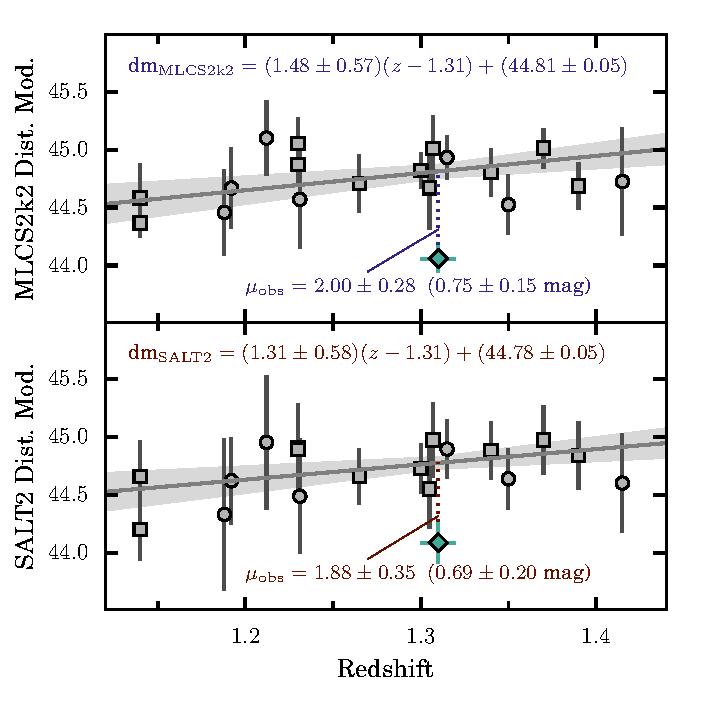
\includegraphics[width=\columnwidth]{FIG/snTomas_hubble_diagram}
\caption{ Measurement of the lensing magnification from comparison of
the \tomas\ distance modulus to a sample of unlensed field SN.
The distance modulus for each SN is derived from light curve fits
using the MLCS2k2 fitter (top panel) and the SALT2 fitter (bottom panel).
\label{fig:MagnificationMeasurement} }
\end{center}
\end{figure}


\section{Discussion}
\label{sec:Discussion}

\subsection{Comparison to Model Predictions}
\label{sec:ComparisonToModelPredictions}

Before the Frontier Fields observations began, the Space Telescope
Science Institute (STScI) issued a call for lens modeling teams to
generate mass models of all 6 Frontier Field clusters, using a shared
collection of all imaging and spectroscopic data available at the
time.  In response to this opportunity, five teams generated eight
models for Abell 2744.  \change{These models necessarily relied on
pre-HFF data, and were required to be complete before the HFF program
began, in order to enable the estimation of magnifications for any new
lensed background sources revealed by the HFF imaging.} An interactive
web tool was created by D. Coe and hosted at STScI, to extract
magnification estimates and uncertainties from each model for any
given redshift and position.  In this work we also consider three
additional models that were created later, taking advantage of new
multiply-imaged galaxies discovered in the HFF imaging as well as new
redshifts for lensed background galaxies.

\begin{deluxetable*}{lccp{1.9in}p{2.2in}}
\tablecolumns{5}
\tablecaption{Predicted magnifications for SN \tomas\ from lens models.\label{tab:PredictedMagnifications}}
\tablehead{ \colhead{Model} & \colhead{Best}\tablenotemark{a} & \colhead{Median\tablenotemark{b}} & \colhead{References} & \colhead{Description}}
\startdata
Sharon(v1)   & 2.53 & 2.57$^{+0.18}_{-0.16}$ & \citealt{Jullo:2007}  & LENSTOOL parametric, strong-lensing based model\\
Sharon(v2)   & 2.73 & 2.69$^{+0.14}_{-0.06}$ &   \citealt{Jullo:2007};\citealt{Johnson:2014} & LENSTOOL parametric, strong-lensing based model\\
CATS-SL      & 2.25 & 2.27$^{+0.05}_{-0.04}$ &   \citealt{Jullo:2009,Jauzac:2012} &  LENSTOOL parametric strong-lensing based model.\\
CATS-SL+WL   & \nodata & 2.62$^{+0.18}_{-0.18}$ & \citealt{Jullo:2009,Jauzac:2012} &  LENSTOOL parametric model with both strong and weak lensing constraints.\\
Jauzac		 & \nodata & 3.37$^{+0.14}_{-0.15}$ &   \citealt{Jauzac:2014,Richard:2014} & Updated version of the CATS-SL model, adds 33 new multiply-imaged galaxies.\\
GLAFIC       & 2.32 & 2.28$^{+0.07}_{-0.11}$ &   \citealt{Oguri:2010,Ishigaki:2015} & Parametric strong-lensing model using the {\tt GLAFIC} code.\tablenotemark{d} \\
Zitrin-NFW   & 2.07 & 2.27$^{+0.23}_{-0.22}$ &   \citealt{Zitrin:2009a} &  Parametric strong-lensing model using PIEMD\tablenotemark{e} profiles for galaxies and NFW\tablenotemark{f} profiles for dark matter halos.\\
Zitrin-LTM   & 2.64 & 2.96$^{+0.77}_{-0.38}$ &   \citealt{Zitrin:2013a} & Parametric strong-lensing model, adopts the Light-Traces-Mass assumption for both the luminous and dark matter.\\
Bradac(v1)   & 3.15 & 2.45$^{+0.19}_{-0.16}$ &   \citealt{Bradac:2005,Bradac:2009} & {\tt SWUnited} : Free-form, strong+weak-lensing based model. Errors from bootstrap resampling only weak-lensing constraints.\\
Bradac(v2)   & 2.21 & 2.23$^{+0.05}_{-0.03}$ &   \citealt{Wang:2015} & \change{Updated version of the {\tt SWUnited} model with new strong-lensing constraints from HFF imaging. Errors from bootstrap resampling only strong-lensing constraints.}\\
Williams     & 2.67 & 2.78$^{+2.68}_{-1.14}$ &   \citealt{Liesenborgs:2006,Liesenborgs:2007,Mohammed:2014} & {\tt GRALE}\tablenotemark{g} : Free-form strong-lensing model using a genetic algorithm.  \\
Merten       & 2.31 & 2.22$^{+0.67}_{-0.19}$ &   \citealt{Merten:2009,Merten:2011} &  {\tt SaWLENS},\tablenotemark{h} Grid-based free-form strong+weak lensing based model using adaptive mesh refinement.\\
Lam			 & \nodata & 2.77$^{+0.36}_{-0.36}$ &   \citealt{Sendra:2014,Lam:2014} & {\tt WSLAP+}\tablenotemark{h} : Free-form model strong-lensing using a grid-based method, supplemented by deflections fixed to cluster member galaxies.\\
Diego\tablenotemark{i}			 & \nodata & 2.10$^{+0.36}_{-0.36}$ &   \citealt{Sendra:2014,Lam:2014} & \change{Alternative implementation of the {\tt WSLAP+}\tablenotemark{h} model, using a different set of strong-lensing constraints and redshifts.}
\enddata
\tablenotetext{a}{The magnification returned for the optimal version of each model, as independently defined by each lens modeling team.}  
\tablenotetext{b}{Median magnification from 100-600 Monte Carlo realizations of the model. Uncertainties enclose 68\%\ of the realized values.}  
\tablenotetext{c}{{\tt LENSTOOL} : \url{http://projects.lam.fr/repos/lenstool/wiki}}
\tablenotetext{d}{{\tt GLAFIC} : \url{http://www.slac.stanford.edu/~oguri/glafic/}}
\tablenotetext{e}{PIEMD: Pseudo Isothermal Elliptical Mass Distrubition}
\tablenotetext{f}{NFW : Navarro-Frenk-White mass density profile \citep{Navarro:1997}.}
\tablenotetext{g}{{\tt GRALE} : GRAvitational LEnsing.}
\tablenotetext{h}{{\tt SaWLENS} : Strong and Weak LENSing analysis code. \url{http://www.julianmerten.net/codes.html}}
\tablenotetext{h}{{\tt WSLAP+} : Weak and Strong Lensing Analysis Package plus member galaxies \change{(Note: no weak-lensing constraints used for Abell 2744)}}
\tablenotetext{i}{\change{No uncertainty estimates were available for the Diego implementation of the {\tt WSLAP+} model, so we adopt the uncertainties from the Lam model.}}
\end{deluxetable*}






\begin{figure}
\begin{center}
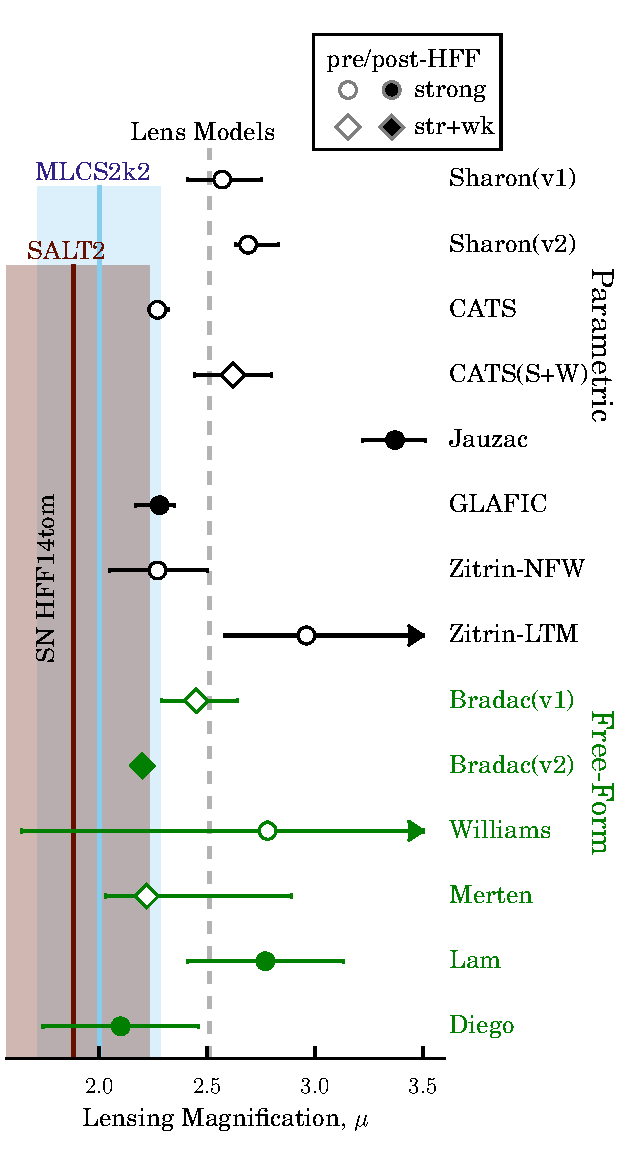
\includegraphics[width=\columnwidth]{FIG/snTomas_magnifications}
\caption{ 
Comparison of the observed lensing magnification to predictions from
lens models. Solid vertical lines show the constraints from SN \tomas\
derived in Section~\ref{sec:Magnification} using the SALT2 (red) and
MLCS2k2 (blue) fitters, with shaded regions marking the total
uncertainty for each. Markers with horizontal error bars show the
median magnification and 68\%\ confidence region from each of the 14
lensing models.  Circles indicate models that use only strong-lensing
constraints, while diamonds denote those that also incorporate
weak-lensing measurements.  Models shown with open markers were
constructed using only data available before the start of the Frontier
Fields observations.  Filled markers indicate models that use
additional input constraints, including new multiply imaged systems
and redshifts.  The eight models shown in black at the top are from
the ``parametric'' family, and the six in green at the bottom are
``free-form.''  Dashed lines mark the unweighted mean of each model
family and shaded regions show the standard error of the mean.
\label{fig:lensingtest} }
\end{center}
\end{figure}

Table~\ref{tab:PredictedMagnifications} lists the \change{14} models,
giving for each one the predicted magnification and uncertainty for a
source at $z=1.31\pm0.01$ and at the position of \tomas.  These models
represent a broad sampling of the techniques and assumptions that can
be applied to the modeling of mass distributions in galaxy clusters. A
rigorous comparison of these disparate lens modeling techniques is
beyond the scope of this work. Table~\ref{tab:PredictedMagnifications}
includes a brief description of each model, but for a complete
discussion of the methodology the reader is referred to the listed
references.

In Figure~\ref{fig:lensingtest} the model predictions are plotted
alongside the observed magnification of SN \tomas, derived in
Section~\ref{sec:Magnification}.  This comparison shows that these 14
models are largely consistent with each other. Naively treating each
model as an independent prediction for the magnification (and ignoring
their quoted uncertainties), one would get a mean for the full sample
of $\mu=2.51\pm0.34$.  This is separated from the observed SN
magnification by $\delta\mu/\mu=27\%$, which is only a 1.2$\sigma$
difference.

The models shown in Figure~\ref{fig:lensingtest} are separated along
the $y$ direction into two broad classes, with 
eight \change{so-called} {\it parametric}\footnote{\change{Although this
nomenclature is becoming standard in the literature, it is somewhat
misleading, as the pixels or grid cells in free-form models are
effectively parameters as well. Perhaps ``simply-parameterized'' would
be more accurate, though we adopt the more common usage here.}}
models on top and six {\it free-form} models on the bottom.
Broadly speaking, the parametric models use parameterized density
distributions to describe the arrangement of mass within the cluster,
typically associating massive dark matter halos with the positions of
bright cluster member galaxies. Therefore, parametric models rely (to
varying degrees) on the assumption that the observed light from
cluster galaxies is a good tracer of the cluster's dark matter.
Free-form models divide the cluster into a grid, generally using a
\change{multi-scale grid} to get better sampling in denser regions. Each grid cell
is assigned a mass or a potential, and then the mass values are
iteratively refined to match the observed lensing
constraints. \change{In some cases an adaptive grid is used so
that the grid spacing itself can also be modified as the model is
iterated \citep[e.g.][]{Liesenborgs:2006,Merten:2009}.}

\change{
In general, free-form methods tend to explore the model parameter
space more fully than parametric methods.  This is reflected in the
size of the error-bars in Figure~\ref{fig:lensingtest}.  For example,
GRALE, which has the largest, and possibly the most realistic
uncertainties is able to account for mass sheet degeneracy by
introducing a free parameter in the reconstruction that represents an
arbitrarily positioned mass sheet, with normalization to be chosen by
the genetic algorithm.  More complex degeneracies are also accounted
for in GRALE through the use of basis
functions \citep{Liesenborgs:2006,Liesenborgs:2007,Mohammed:2014} }

Figure~\ref{fig:lensingtest} also separates the models based on the
scope of input data constraints used.  Ten of the models rely only
on strong-lensing constraints (plotted as circles), while the other
four also use weak-lensing measurements (diamonds).  Ten of the
models were constructed using only pre-HFF data (open symbols), and
four others added new multiply-imaged systems and redshifts.

In spite of the great variety in input data and methodology, these
lens models overall are delivering consistent and fairly accurate
estimates of the magnification.  \change{Six of the tested models
(CATS, GLAFIC, Zitrin-NFW, Bradac(v2), Merten, Diego) report a median
value that falls within the 1$\sigma$ uncertainty range of the
measured magnification, and two of the free-form models (Williams,
Diego) report uncertainties that overlap the central $\mu$ as measured
from both of the SN light curve fitters.}  Furthermore, the scatter
amongst models provides a reasonable estimate of the magnification
uncertainty.

This is largely in agreement with the results
of \citetalias{Patel:2014} and \citet{Nordin:2014}.  The fact that the
model predictions are collectively within $2\sigma$ of the observed
magnification is especially encouraging for these Abell 2744
models. This is a merging cluster with a complex mass distribution,
and most of the models we are evaluating are preliminary products,
generated quickly and without access to the rich data from the
Frontier Fields program.

However, beyond this first-order agreement, there is a systematic bias
apparent. All of the lens models \change{return median magnifications
that are} {\it higher} than the observed value, and \change{half of
the models are discrepant by more than $1\sigma$.}  It is important to
emphasize that SN \tomas\ only samples a single sight-line through the
cluster, so any conclusions to be drawn from this analysis are
necesssarily limited.  Nevertheless, a systematic shift common to all
models is surprising, given the wide range of modeling strategies,
input data, and physical assumptions represented by this set of
models.  In the following subsections we examine possible explanations
for this \change{small but} apparently universal bias.

\subsection{Nearby Cluster Member Galaxy}
\label{sec:NearbyClusterMemberGalaxy}

The line of sight to SN \tomas\ is 5\farcs8 from a bright cluster
member galaxy, due North of the SN position (see
Figure~\ref{fig:DiscoveryImage}).  If the mass-to-light ratio (M/L)
for this galaxy were significantly different from the M/L for other
cluster member galaxies, then its proximity to the SN sight-line could
introduce a bias in the magnification.  This bias might be
particularly acute for models that make a strict ``light traces mass''
assumption, such as the Sharon, CATS, Jauzac, GLAFIC and Zitrin-LTM
models.  

We tested this hypothesis using the Jauzac model by allowing the mass
of the nearby cluster member galaxy to vary as a free parameter in the
model. We found that the change in the SN \tomas\ magnification
prediction was less than $\Delta\mu=0.1$.  This additional dispersion
is already included in the uncertainties quoted for that model in
Table~\ref{tab:PredictedMagnifications} and
Figure~\ref{fig:lensingtest}.  Furthermore, an erroneous M/L
value for the nearby cluster member galaxy could not explain the
systematic shift of all lens models, because some do not incorporate
cluster member galaxies into their constraints at all (the free-form
Bradac, Williams and Merten models).

\subsection{Sparse Strong Lensing Constraints}
\label{sec:SparseStrongLensingConstraints}

At the outset of the HFF survey, only 33 multiply-imaged galaxies
behind Abell 2744 were known.  One might expect that the addition of
new lensing constraints from the HFF data would improve the model
constraints and reduce the tension between the predicted and observed
magnification.  However, for \changeG{two} of the most recent
models \citep{Jauzac:2014c,Lam:2014} that include new strong-lensing
constraints, the predicted magnification is still significantly higher
than the observed value.  Again the CATS model family provides a
useful case study.  The Jauzac model shares the same lens modeling
software (LensTool), and the same primary methodology as the earlier
CATS models.  A key difference is that the Jauzac model incorporates
many new multiply imaged galaxies and corrects a mis-identified
multiply-imaged system near the SN \tomas\ position.  These
improvements should in principle make the Jauzac model magnification
estimates more accurate, though we in fact see the opposite result:
the Jauzac model predicts a $\mu$ that is higher than the measured
value by \changeG{$4.3\sigma$.}

This shift to higher magnifications is not, however, unique to the
SN \tomas\ position.  \citet{Jauzac:2014c} noted that their updated
mass model of Abell 2744 results in a systematic increase in the
magnification values across the cluster field. Examining a sample of
$\sim$30 multiple images, \citeauthor{Jauzac:2014c} found that the
magnifications increased by a factor of $\sim1.5$ relative to pre-HFF
models.  Although this single sight-line can only provide a very
limited test of the model, the \changeG{$4.3\sigma$} discrepancy is at
least a strong suggestion that improving the number and quality of
strong-lensing constraints can still lead to magnification maps that
are susceptible to systematic biases.

\change{
\subsection{Misidentification of System 3}
\label{sec:MisidentificationOfSystem3}
}

\begin{figure}
\begin{center}
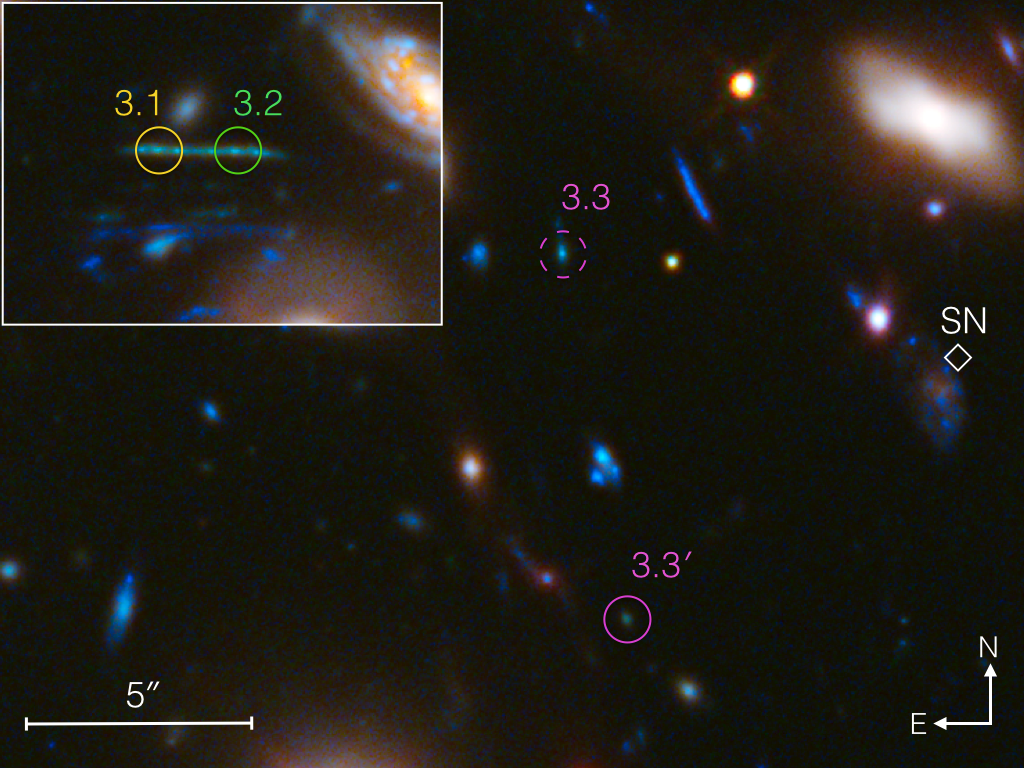
\includegraphics[width=\columnwidth]{FIG/system3.png}
\caption{ 
The disputed component of the multiply-imaged galaxy System 3. The
original position, as given in \citet{Merten:2011} is marked with a
dashed magenta circle labeled 3.3. The solid magenta circle shows the
revised location as proposed in \citet{Jauzac:2014c}.  Both positions
are $\sim$10\arcsec\ from the SN location.  The inset panel shows the
other two components of this multiply-imaged system, 3.1 and 3.2 (on
the same scale as the main panel), which are located north-east of the
cluster center.
\label{fig:system3} }
\end{center}
\end{figure}

\change{
It is important to note that in regards to the impact on this
particular sight-line, not all strong-lensing constraints are equal.
An error in the association of multiple images or in the redshift of a
multiply-imaged galaxy would have a more significant impact if that
system has a projected position close to our SN
sight-line \changeG{\citep[see][for a quantitative assessment of this
effect]{Johnson:2014}.}  It happens that there is one such system, for
which the position of a multiple image near SN \tomas\ is presently
disputed.  }

\change{
This multiply-imaged galaxy was originally labeled as {\it System 3}
in \citet{Merten:2011}.  As shown in Figure~\ref{fig:system3}, it is
stretched into two adjacent arcs northeast of the cluster core (images
3.1 and 3.2), with a third image on the western edge of the
strong-lensing region (image 3.3 at 00:14:18.595,
-30:23:58.42).  \citet{Richard:2014} echoed this initial
identification in producing the {\tt CATS} models, which we cite in
Table~\ref{tab:PredictedMagnifications} and
Figure~\ref{fig:lensingtest}.  In developing the {\tt Sharon-v2}
models, \citet{Johnson:2014} provided a secure spectroscopic
constraint of $z=3.98\pm0.02$ for this system, based on a spectrum of
the combined 3.1+3.2 source. The identification of the original image
3.3 has been called into question by two independent analyses.  Using
HFF imaging data, \citet{Lam:2014} suggested an alternative third
image for this system roughly 8\arcsec\ to the south, which we will
call \33p\ (00:14:18.39, -30:24:06.53).
However, \citeauthor{Lam:2014} rejected this possibility based on a
difference in colors between \33p\ and images 3.1 and 3.2.  In
contrast, \citeauthor{Jauzac:2014c} argue that the position \33p\
is correct, and find that reassigning this multiple image results in a
tighter model reconstruction for the locations of other
multiply-imaged systems in the vicinity.
}

\change{
Resolving the identification of this single multiply-imaged galaxy
could be a component in resolving the magnification
discrepancy, though it is unlikely to completely remove the tension.
It is true that the model that reassigns the position to \33p\
({\tt Jauzac}) is also the one with the largest deviation from our
observed $\mu$ value.  However, \citet{Jauzac:2014c} have already
evaluated the impact of relocating this single source, and
they find that it is not responsible for the observed increase in
magnifications across the field. Rather, the 
primary cause for the general magnification increase is the addition
of new multiple images in the Northern region, detected using the new
HFF data. } 

\subsection{Mass Profile Extrapolation}
\label{sec:MassProfileExtrapolation}

Eight of the mass models evaluated here are constrained only using
strong-lensing features such as multiply-imaged background galaxies
and highly magnified arcs.  There are now $\sim$150 known lensed
images behind Abell 2744 \citep{Jauzac:2014c}, but SN \tomas\ is
located several arcseconds outside the core region of the cluster
where these multiply-imaged galaxies are found.  Therefore these eight
``strong-lensing only'' models must necessarily rely on extrapolations
to provide a prediction for the SN \tomas\ magnification.  Let us
suppose that the true cluster density profile for Abell 2744 happens
to have a sharp drop right at the edge of this core strong-lensing
region. In that case these eight models might well overestimate the
mass interior to the \tomas\ position, and thus systematically
overestimate the magnification.

The other three models in our comparison set also use the strong
lensing constraints from the core region, but additionally utilize
weak lensing measurements to provide additional constraints on the
mass distribution farther from the cluster core.  The signal from weak
lensing relies on a large sample of background galaxies, so this
constraint operates principally at separations more than 1\arcmin\ from
the cluster core.  At a projected separation of $\sim40\arcsec$,
SN \tomas\ falls in between the strong- and weak-lensing regimes, and
one would expect that models incorporating both of those constraints
would be less susceptible to the systematic bias of a sharply
steepening mass profile.  The lowest magnification estimate in our
sample (from the Merten model) is among this sub-sample.  However, we
find that collectively these three strong+weak models (shown as
diamonds in Figure~\ref{fig:lensingtest}) exhibit the same propensity
to overestimate the magnification along this line of sight.  Thus, a
sudden change in the mass profile outside the strong lensing region is
not a likely explanation for this small systematic bias.

With two versions of the CATS model, we also have a more direct test
of the effect of introducing weak lensing constraints.  The initial
CATS model uses only strong-lensing constraints, and gives
$\mu=2.27^{+0.05}_{-0.04}$, slightly higher than the measured value.
A second iteration of this model, labeled here as CATS-SL+WL, used the
same strong-lensing features, but added in weak lensing constraints.
The revised magnification of $\mu=2.62\pm0.18$ is further from the
measured value, which serves to reinforce the conclusion that adding
weak lensing constraints cannot, by itself, resolve this bias.


\subsection{Redshift Error}
\label{sec:RedshiftError}

\change{
If the redshift of the SN derived in Section~\ref{sec:Spectroscopy}
were incorrect, then one would derive a different value for the
magnification, both from the SN measurement and the lens model
predictions.  Conceivably, this could resolve the tension between the
measurement and the models.  It is often the case in SN surveys that
redshifts are assigned based on a host galaxy association, typically
inferred from the projected separation between the SN and nearby
galaxies.  In this case the redshift evidence comes from the SN
itself, and we find a consistent redshift from both the SN spectrum
(Section~\ref{sec:SpecRedshift}) and the light curve
Section~\ref{sec:PhotometricClassification}, which are both within the
$1\sigma$ range of the photometric redshift for the nearest detected
galaxy: $z=1.5\pm0.2$. This appears to be a solid and self-consistent
picture, so the evidence strongly disfavors any redshift that is
significantly different from $z=1.3$.
}

\change{
We have adopted the spectroscopic redshift of $z=1.31\pm0.01$ for the
magnification comparison.  Spectroscopic SN redshifts are generally more
precise and accurate than those derived from SN
photometry \citep{Rodney:2010b,Kessler:2010,Sako:2011}.  However, in
this case the spectrum is limited to the rest-frame near-UV
wavelengths, where the available SN spectral template libraries are
more limited than at optical wavelengths.  If we use the photometric
redshift of $z=1.35\pm0.02$ instead, then the measured magnification
is reduced.\footnote{By increasing the redshift, the SN is presumed to
be at a greater distance, so to first order one would be expect it to
appear slightly fainter (larger distance modulus). If the distance
modulus inferred from the light curve fit remained constant, this
would drive the inferred magnification to a higher value.  However,
the light curve fitting is more strongly affected by the covariance
between redshift, color, and light curve width.  In this case, these
effects drive the distance modulus to a larger value at $z=1.35$,
resulting in a smaller value of the observed magnification $\mu$.}
From the SALT2 fitter we derive $\mu_{\rm SALT2}=1.80\pm0.30$ and from
MLCS2k2 we get $\mu_{\rm MLCS2k2}=1.83\pm0.17$.  The lens models are
also shifted, and they uniformly move in the opposite direction, to
magnification values that are {\it larger} than at $z=1.31$, by
$\sim1$\%.  Thus, shifting the SN to the photometric redshift of
$z=1.35$ only serves to (slightly) exacerbate the tension between the
observations and models.  }


\subsection{Foreground Dust}
\label{sec:ForegroundDust}

\change{
All SN sight-lines must intersect some amount of foreground dust from
the immediate circumstellar environment, the host galaxy, and the
intergalactic medium (IGM). In the case of SN \tomas\ one might posit
some dust extinction from the intra-cluster medium (ICM) of Abell
2744, although measurements of rich clusters suggest that the ICM has
only a negligible dust
content \citep{Maoz:1995,Stickel:2002,Bai:2007}.  When fitting
the \tomas\ light curve we account for dust by including corrections
that modify the inferred luminosity distance based on the SN color.
If after applying these dust corrections we are still {\it
underestimating} the effect of dust along this sight-line, then the SN
would appear more dim, the inferred distance modulus would be higher,
and the measured magnification would be reduced -- consistent with the
discrepancy we observe.  
}

\change{
In Section~\ref{sec:LightCurveFitting} we found that SN \tomas\ is on
the blue end of the normal range of Type Ia SN colors.  With the SALT2
fitter we measured a color parameter $c=-0.115\pm0.025$, and with
MLCS2k2 we found the host galaxy dust extinction to be $A_{\rm
V}=0.014\pm0.037$ magnitudes.  These colors are tightly constrained,
as we are fitting to photometry that covers a rest-frame wavelength
range from $\sim3500-7000$\AA\ and extends to $\sim$30 days past
maximum brightness.  This leaves little room for the luminosity
measurement to be biased by dust, as the dimming of \tomas\ would also
necessarily be accompanied by some degree of reddening. 
}

\change{
Nevertheless, one might suppose that a bias could be introduced if we
have adopted incorrect values for the color correction parameter
$\beta$ or extinction law $R_V$ in the SALT2 and MLCS2k2 fits,
respectively.  The appropriate value to use for this color correction
and how it affects inferences about the intrinsic scatter in Type Ia
SN luminosities is a complex question that is beyond the scope of this
work \citep[see
e.g.][]{Marriner:2011,Chotard:2011,Kessler:2013,Scolnic:2014a}.
However, we can already rule this out as a solution for the
magnification discrepancy.  Our error on the \tomas\ distance modulus
already includes an uncertainty in the extinction law and a related
error to account for the intrinsic luminosity scatter. These are well
vetted paraemeters, based on observations of $\sim500$ SNe extending
to $z\sim1.5$ \citep{Sullivan:2011}.  Furthermore, there is no reason
to propose that SN \tomas\ is uniquely affected by a peculiar type of
dust.  Thus, any change in the color correction applied to SN \tomas\
would require the same adjustment to be applied to the unlensed SNe at
similar redshift that make up our comparison sample, largely negating
the effect on the inferred magnification.  }

\change{
The traditional color corrections as formalized in SN light curve
fitters are designed to account for a dust component that lies in the
rest frame of the SN.  The inferred luminosity of a SN can also be
affected by the presence of foreground dust with a different redshift
and possibly a different reddening law \citep{Menard:2010b}.  However,
the magnitude of such a bias is insufficient to account for the
observed discrepancy, \citet{Menard:2010a} estimate the opacity of the
universe as $\langle A_{V}\rangle\sim0.03$ mag up to $z=0.5$.  While
this can have a measurable impact on precise cosmological constraints,
it is far less than the 0.25 mag difference between the observed
magnification of \tomas\ and the mean of the model predictions.  
}


\subsection{Misclassification}
\label{sec:Misclassification}

\begin{figure}
\begin{center}
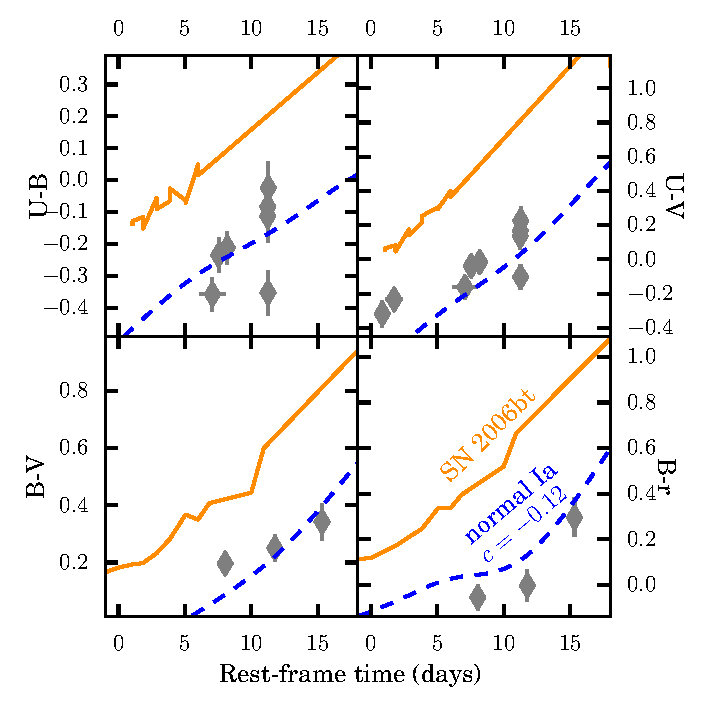
\includegraphics[width=\columnwidth]{FIG/snTomas_sn06bt_colorcurves}
\caption{ 
Comparing \tomas\ observations to the color curves of SN 2006bt and a
normal Type Ia SN model. Grey points show the observed colors of
SN \tomas, k-corrected to rest-frame UBVr bands. Solid orange lines
show the observed color curves for the peculiar Type Ia SN
2006bt. Dashed blue lines show the color curves for a normal Type Ia
SN, derived from the SALT2 model with a color parameter $c=-0.12$, set
to match the best-fit color for SN \tomas.
\label{fig:colorcomparison} }
\end{center}
\end{figure}

\change{
Is it possible that \tomas\ is an example of a peculiar stellar
explosion that does not follow the relationship between light curve
shape and luminosity observed in normal Type Ia SNe?  In
Sections~\ref{sec:SNID} and \ref{sec:PhotometricClassification} we
classified SN Tomas as a normal Type Ia SN based on both the
spectroscopic and photometric evidence.  This rules out the
possibility that \tomas\ belongs to a different class of normal SN
explosions (Type Ib, Ic, or II). In
Section \ref{sec:LightCurveFitting} we fit the \tomas\ light curve to
determine a luminosity distance and found that the light curve shape
and color are consistent with a Type Ia SN of average light curve
width, with minimal dust extinction.  This excludes the possibility
that \tomas\ is one of the sub-class of faint and fast-declining Type
Ia SNe like SN 1991bg.  }

\change{
One remaining possibility is that \tomas\ could be part of a rare
sub-category of peculiar Type Ia SNe that masquerade as their normal
cousins, epitomized by the prototype SN 2006bt \citep{Foley:2010}.
These objects appear to have a normal Type Ia light curve shape,
except for the absence of a secondary maximum or ``shoulder'' in
near-IR bands.  The reddest filter available for the \tomas\ light
curve is F160W, which has an effective rest-frame wavelength of
6623\AA\ at $z=1.31$, making it close to the rest-frame {\it r} band.
Although the near-IR shoulder is more prominent in the rest-frame {\it
i} band, we can see in Figures~\ref{fig:LightCurveFits} that the F160W
light curve may suggest a weak or delayed near-IR shoulder.  The
second-to-last observation in F160W is $\sim1\sigma$ lower than
predicted by the best-fit SALT2 and MLCS2k2 models. This is tenuous
evidence, but it would be consistent with a 2006bt-like light curve.
}

\change{
In this case, however, the color of SN \tomas\ can rule out a
classification as a 2006bt-like object.  All members of this peculiar
sub-class exhibit very red colors across all optical and near-IR
bands, consistent with a very cool photosphere \citep{Foley:2010}.
Figure~\ref{fig:colorcomparison} shows that \tomas\ is bluer than the
SN 2006bt prototype by at least 0.25 magnitudes in every color. The
observed \tomas\ colors are fully consistent with the a normal, blue
Type Ia SN (the SALT2 model is shown).
}

\section{Summary and Conclusions}
\label{sec:SummaryAndConclusions}

The appearance of a Type Ia SN behind a massive galaxy cluster
provides a rare opportunity to use a standard candle for a direct
measurement of the absolute magnification due to gravitational
lensing.  The discovery of SN \tomas\ in the HFF imaging of Abell 2744
offers the first chance to apply this test on a cluster with multiple
publicly-available lens models.  We have found that the spectrum and
light curve of SN \tomas\ are well matched by templates of a normal
Type Ia SN at $z=1.31\pm0.01$.  Using the two most prevalent \SNIa\
light curve fitters, SALT2 and MLCS2k2, we get a consistent
measurement of the distance modulus
(Table~\ref{tab:MeasuredMagnification}).  Using a
cosmology-independent comparison against a sample of unlensed \SNeIa\
at similar redshifts, we find that SN \tomas\ is $\sim0.7$ magnitudes
brighter than the field sample would predict.  Attributing this
difference to the gravitational lensing magnification (and accounting
for the intrinsic scatter in luminosity of the \SNIa\ population), we
have derived a consistent measured magnification of $\mu_{\rm
SALT2}=1.88\pm0.35$.  $\mu_{\rm MLCS2k2}=2.00\pm0.28$, from the two
light curve fitters.

Taking advantage of the availability of eleven well-constrained lens
models for the Abell 2744 cluster, we have used SN \tomas\ to ask
how accurately these lens models can predict the magnification along
this line of sight.   We find that these models are consistent, and
fairly accurate, collectively predicting $\mu=2.60\pm0.34$.  This is
encouraging, and reinforces the quality and value of these public lens
models for studying magnified background objects.   However, the fact
that all models predict a larger magnification value than we observe
is an indication that there is a small systematic bias inherent to
this cluster or sight-line. 

We have speculated on the origin of this systematic bias,
evaluating six possible causes: 

\begin{enumerate}
\item The close proximity of a cluster member galaxy is leading to a
biased magnification, because that galaxy's M/L is atypical.
\item The models are limited by a scarcity of strong lensing constraints
\item The cluster mass profile exhibits a sudden change outside of the core
strong-lensing region, where we lack multiply-imaged background
sources to constrain it. 
\item \change{The redshift assigned to SN \tomas\ is in error.}
\item \change{SN \tomas\ is dimmed by foreground dust.}
\item \change{SN \tomas\ is not a normal Type Ia SN.}
\end{enumerate}

\noindent The first three of these take on the discrepancy from 
the lens modeling side, but none are completely satisfactory. For each
of these scenarios, we would expect that certain subsets of the
available lens models would be less sensitive to the proposed
systematic bias.  However, the small discrepancy between the predicted
and observed lensing magnification is persistent when we bifurcate the
sample of lens models according to methodology (parametric
vs. free-form), number of strong-lensing constraints (pre- vs
post-HFF), and scope of lensing constraints (strong-lensing only
vs. strong+weak). Thus, comparison of the available models does not
provide any definitive explanation for this magnification tension.

\changeG{
At least for this particular sight-line, the free-form models perform
better both in the sense that the mean and standard error for this
subset ($2.34\pm0.27$) is closer to the measured value ($2.00\pm0.28$)
than is the parametric set ($2.59 +- 0.36$).  These free-form models
also deliver more realistic uncertainties (with the exception of the
Bradac(v2) model -- see \citet{Wang:2015} for further discussion of
the changes made from v1 to v2 of that model).  This may indicate that
the free-form approach in general is more successful in capturing the
uncertainty from biases inherent to the mass modeling exercise, such
as the mass sheet degeneracy and more complex ``approximate
invariances'' \citep{Liesenborgs:2012,Schneider:2014}.  It may also be
the case that the greater flexibility of the free-form models makes
them better suited for predicting magnifications of sources that fall
outside the strong-lensing region -- such as SN \tomas.  }

\change{
The last three possible explanations presume an error in the
interpretation of the available SN data.  We reject the possibility
that a redshift error is the primary cause of the discrepancy, as the
redshift evidence is derived principally from the SN itself and not
from the host galaxy. A value of $z\sim1.3$ is well supported by both
the spectroscopic and photometric SN data, and changing the redshift
within the constraints of these complementary observations only serves
to increase the tension between the observed and predicted
magnifications.  We also find it implausible that there is sufficient
dust in the cluster or elsewhere along the line of sight to account
for the magnification discrepancy.  A dust-induced bias is also
disfavored by the very blue color of SN \tomas.  }

\change{
Finally, we have considered whether the SN could be
mis-classified. Once again the combination of spectroscopic and
photometric evidence strongly supports our classification of
SN \tomas\ as a normal Type Ia SN.  The most plausible
mis-classification would be that the object is a peculiar Type Ia of
the SN 2006bt-like sub-class.  Although the light curve shape could
allow this possibility, the blue color of \tomas\ can once again
reject this alternative. 
}

This single object behind a single cluster is not in and of itself a
cause for alarm.  Previous analyses of lensed \SNIa\ found no
significant discrepancy beween the observed \SNIa\ magnifications and
the predictions from lens models
(\citetalias{Patel:2014}; \citealt{Nordin:2014}), albeit with a much
smaller set of lens models being tested.  The observed systematic bias
for \tomas\ is small, and many of the lens models being evaluated are
preliminary models that have not been updated to include all of the
HFF data.  Future revisions of the lens models for Abell 2744 should
either incorporate the observed magnification of \tomas\ as a new
model constraint, or can revisit this test to evaluate whether the
bias persists.

\change{
A promising avenue for exploring the origins of systematic biases in
cluster lens models is through the use of simulated data.  One can
start with very deep high-resolution multi-band imaging on an unlensed
field that has a fairly complete spectroscopic redshift catalog, such
as the Hubble Ultra Deep Field.  Then a simulated galaxy cluster is
placed in the field, and the background galaxies are distorted into
arcs and multiple images using a well-defined lensing prescription.
The artificially lensed images can then be distributed to lens
modeling teams who attempt to reconstruct the (known) mass profile of
the simulated cluster.  This exercise has recently been pursued with a
set of synthetic clusters similar to those observed in the HFF program
(Meneghetti et al. in prep).  Preliminary analysis of this simulation
comparison suggests that \changeG{magnifications tend to be
overestimated} for sources that lie outside the strong-lensing region
along the minor axis direction of an elongated cluster.  Our analysis
of SN \tomas\ here indicates that such simulation efforts will be an
important step for moving toward precision science with cluster-lensed
sources.  }

Increasing the sample of SNe behind clusters \changeG{like those in
the HFF program -- with rich lensing constraints and deep imaging -- }
would allow this test to be repeated and refined.  With 10 or 100 such
objects, it would be possible to see whether the SN \tomas\ $\mu$
discrepancy is simply an outlier, or an indication of a more
pernicious systematic error.  Any cluster that has been vetted by
pencil-beam magnification tests using lensed \SNIa\ will be able to
provide a more reliable measure of the magnifications for very high
redshift objects.  Similarly, a broad sample of SNe like \tomas\ would
help to define the preferred lens modeling methodology by highlighting
any models that consistently perform well in \SNIa\ lensing tests.
The ongoing FrontierSN program will discover and follow any more
highly magnified SNe that appear behind the Frontier Field
clusters. Unfortunately, the HFF survey is not designed with high-z
transient discovery as a primary science goal, so the FrontierSN
effort will likely add no more than 1-3 new lensed \SNIa. Further
imaging of strong-lensing clusters with \HST\ or the James Webb Space
Telescope (JWST) could enable a larger sample to be collected,
especially if the filters and cadence are optimized for detection
of \SNIa\ at $z>1$.  Massive clusters such as Abell 2744 will continue
to be attractive as cosmic telescopes, allowing the next generation of
telescopes to reach the faintest objects in the very early universe.
The puzzling bias revealed by SN \tomas\ supports a concerted effort
to improve these lenses with \change{further examination of lensing
systematics through simulations and collection of} a larger sample of
magnified SNe.


\bigskip


{\bf Acknowledgments:}

This work is dedicated to our colleague and friend Tomas Dahlen, for
whom this supernova has been named in memorium. He is dearly missed.

We thank the Hubble Frontier Fields team at STScI
for their substantial efforts to make the HFF program successful.  In
particular, thanks are due to Matt Mountain for the allocation of
discretionary orbits for the HFF program; to Jennifer Lotz, Norman
Grogin and Patricia Royle for accommodations in strategy and
implementation to make the FrontierSN program possible; and to Dan Coe
for curating the excellent and accessible lens model comparison tools.
We also must thank the CLASH team, led by Marc Postman, for
observations, catalogs, and high level science products that were of
significant value for this analysis.

Financial support for this work was provided to SAR by NASA through grants
HST-HF-51312 and HST-GO-13386 from the Space Telescope
Science Institute, which is operated by Associated Universities for
Research in Astronomy, Inc., under NASA contract NAS 5-26555.

AM acknowledge the financial support of the Brazilian funding agency
FAPESP (Post-doc fellowship - process number 2014/11806-9)

Support for this research at Rutgers University was provided in part
by NSF CAREER award AST-0847157 to SWJ.  The Dark Cosmology Centre is
supported by the Danish National Research Foundation.

J.M.D acknowledges support of the consolider project CAD2010-00064 and
AYA2012-39475-C02-01 funded by the Ministerio de Economia y
Competitividad.

J.M. contributed to this research from the Jet Propulsion Laboratory,
California Institute of Technology, under a contract with NASA and
acknowledges support from NASA Grants HST-GO-13343.05-A and
HST-GO-13386.13-A. The research leading to these results has received
funding from the People Programme (Marie Curie Actions) of the European
Union's Seventh Framework Programme (FP7/2007-­2013) under REA grant
agreement number 627288.

{\it Facilities:} \facility{HST (WFC3)}
\smallskip

\bibliographystyle{apj}
\bibliography{bibdesk}

\end{document}

